% Options for packages loaded elsewhere
% Options for packages loaded elsewhere
\PassOptionsToPackage{unicode}{hyperref}
\PassOptionsToPackage{hyphens}{url}
%
\documentclass[
  ignorenonframetext,
  aspectratio=169,
  t]{beamer}
\newif\ifbibliography
\usepackage{pgfpages}
\setbeamertemplate{caption}[numbered]
\setbeamertemplate{caption label separator}{: }
\setbeamercolor{caption name}{fg=normal text.fg}
\beamertemplatenavigationsymbolsempty
% remove section numbering
\setbeamertemplate{part page}{
  \centering
  \begin{beamercolorbox}[sep=16pt,center]{part title}
    \usebeamerfont{part title}\insertpart\par
  \end{beamercolorbox}
}
\setbeamertemplate{section page}{
  \centering
  \begin{beamercolorbox}[sep=12pt,center]{section title}
    \usebeamerfont{section title}\insertsection\par
  \end{beamercolorbox}
}
\setbeamertemplate{subsection page}{
  \centering
  \begin{beamercolorbox}[sep=8pt,center]{subsection title}
    \usebeamerfont{subsection title}\insertsubsection\par
  \end{beamercolorbox}
}
% Prevent slide breaks in the middle of a paragraph
\widowpenalties 1 10000
\raggedbottom
\AtBeginPart{
  \frame{\partpage}
}
\AtBeginSection{
  \ifbibliography
  \else
    \frame{\sectionpage}
  \fi
}
\AtBeginSubsection{
  \frame{\subsectionpage}
}
\usepackage{iftex}
\ifPDFTeX
  \usepackage[T1]{fontenc}
  \usepackage[utf8]{inputenc}
  \usepackage{textcomp} % provide euro and other symbols
\else % if luatex or xetex
  \usepackage{unicode-math} % this also loads fontspec
  \defaultfontfeatures{Scale=MatchLowercase}
  \defaultfontfeatures[\rmfamily]{Ligatures=TeX,Scale=1}
\fi
\usepackage{lmodern}

\ifPDFTeX\else
  % xetex/luatex font selection
\fi
% Use upquote if available, for straight quotes in verbatim environments
\IfFileExists{upquote.sty}{\usepackage{upquote}}{}
\IfFileExists{microtype.sty}{% use microtype if available
  \usepackage[]{microtype}
  \UseMicrotypeSet[protrusion]{basicmath} % disable protrusion for tt fonts
}{}
\makeatletter
\@ifundefined{KOMAClassName}{% if non-KOMA class
  \IfFileExists{parskip.sty}{%
    \usepackage{parskip}
  }{% else
    \setlength{\parindent}{0pt}
    \setlength{\parskip}{6pt plus 2pt minus 1pt}}
}{% if KOMA class
  \KOMAoptions{parskip=half}}
\makeatother

\usepackage{color}
\usepackage{fancyvrb}
\newcommand{\VerbBar}{|}
\newcommand{\VERB}{\Verb[commandchars=\\\{\}]}
\DefineVerbatimEnvironment{Highlighting}{Verbatim}{commandchars=\\\{\}}
% Add ',fontsize=\small' for more characters per line
\usepackage{framed}
\definecolor{shadecolor}{RGB}{241,243,245}
\newenvironment{Shaded}{\begin{snugshade}}{\end{snugshade}}
\newcommand{\AlertTok}[1]{\textcolor[rgb]{0.68,0.00,0.00}{#1}}
\newcommand{\AnnotationTok}[1]{\textcolor[rgb]{0.37,0.37,0.37}{#1}}
\newcommand{\AttributeTok}[1]{\textcolor[rgb]{0.40,0.45,0.13}{#1}}
\newcommand{\BaseNTok}[1]{\textcolor[rgb]{0.68,0.00,0.00}{#1}}
\newcommand{\BuiltInTok}[1]{\textcolor[rgb]{0.00,0.23,0.31}{#1}}
\newcommand{\CharTok}[1]{\textcolor[rgb]{0.13,0.47,0.30}{#1}}
\newcommand{\CommentTok}[1]{\textcolor[rgb]{0.37,0.37,0.37}{#1}}
\newcommand{\CommentVarTok}[1]{\textcolor[rgb]{0.37,0.37,0.37}{\textit{#1}}}
\newcommand{\ConstantTok}[1]{\textcolor[rgb]{0.56,0.35,0.01}{#1}}
\newcommand{\ControlFlowTok}[1]{\textcolor[rgb]{0.00,0.23,0.31}{\textbf{#1}}}
\newcommand{\DataTypeTok}[1]{\textcolor[rgb]{0.68,0.00,0.00}{#1}}
\newcommand{\DecValTok}[1]{\textcolor[rgb]{0.68,0.00,0.00}{#1}}
\newcommand{\DocumentationTok}[1]{\textcolor[rgb]{0.37,0.37,0.37}{\textit{#1}}}
\newcommand{\ErrorTok}[1]{\textcolor[rgb]{0.68,0.00,0.00}{#1}}
\newcommand{\ExtensionTok}[1]{\textcolor[rgb]{0.00,0.23,0.31}{#1}}
\newcommand{\FloatTok}[1]{\textcolor[rgb]{0.68,0.00,0.00}{#1}}
\newcommand{\FunctionTok}[1]{\textcolor[rgb]{0.28,0.35,0.67}{#1}}
\newcommand{\ImportTok}[1]{\textcolor[rgb]{0.00,0.46,0.62}{#1}}
\newcommand{\InformationTok}[1]{\textcolor[rgb]{0.37,0.37,0.37}{#1}}
\newcommand{\KeywordTok}[1]{\textcolor[rgb]{0.00,0.23,0.31}{\textbf{#1}}}
\newcommand{\NormalTok}[1]{\textcolor[rgb]{0.00,0.23,0.31}{#1}}
\newcommand{\OperatorTok}[1]{\textcolor[rgb]{0.37,0.37,0.37}{#1}}
\newcommand{\OtherTok}[1]{\textcolor[rgb]{0.00,0.23,0.31}{#1}}
\newcommand{\PreprocessorTok}[1]{\textcolor[rgb]{0.68,0.00,0.00}{#1}}
\newcommand{\RegionMarkerTok}[1]{\textcolor[rgb]{0.00,0.23,0.31}{#1}}
\newcommand{\SpecialCharTok}[1]{\textcolor[rgb]{0.37,0.37,0.37}{#1}}
\newcommand{\SpecialStringTok}[1]{\textcolor[rgb]{0.13,0.47,0.30}{#1}}
\newcommand{\StringTok}[1]{\textcolor[rgb]{0.13,0.47,0.30}{#1}}
\newcommand{\VariableTok}[1]{\textcolor[rgb]{0.07,0.07,0.07}{#1}}
\newcommand{\VerbatimStringTok}[1]{\textcolor[rgb]{0.13,0.47,0.30}{#1}}
\newcommand{\WarningTok}[1]{\textcolor[rgb]{0.37,0.37,0.37}{\textit{#1}}}

\usepackage{longtable,booktabs,array}
\newcounter{none} % for unnumbered tables
\usepackage{calc} % for calculating minipage widths
\usepackage{caption}
% Make caption package work with longtable
\makeatletter
\def\fnum@table{\tablename~\thetable}
\makeatother
\usepackage{graphicx}
\makeatletter
\newsavebox\pandoc@box
\newcommand*\pandocbounded[1]{% scales image to fit in text height/width
  \sbox\pandoc@box{#1}%
  \Gscale@div\@tempa{\textheight}{\dimexpr\ht\pandoc@box+\dp\pandoc@box\relax}%
  \Gscale@div\@tempb{\linewidth}{\wd\pandoc@box}%
  \ifdim\@tempb\p@<\@tempa\p@\let\@tempa\@tempb\fi% select the smaller of both
  \ifdim\@tempa\p@<\p@\scalebox{\@tempa}{\usebox\pandoc@box}%
  \else\usebox{\pandoc@box}%
  \fi%
}
% Set default figure placement to htbp
\def\fps@figure{htbp}
\makeatother





\setlength{\emergencystretch}{3em} % prevent overfull lines

\providecommand{\tightlist}{%
  \setlength{\itemsep}{0pt}\setlength{\parskip}{0pt}}



 


\setbeamertemplate{frametitle continuation}{}
\setbeamertemplate{itemize items}[circle]
\usepackage{caption}
\usepackage{textpos}
\setlength{\TPHorizModule}{1cm}
\setlength{\TPVertModule}{1cm}

% credit line
\newcommand{\credit}{\scriptsize\textcolor{gray!70!black}{\quad courtiol@izw-berlin.de | \url{www.datazoogang.de} | \url{www.izw-berlin.de/en}}}

% create footer with slide number
\setbeamertemplate{footline}{%
  \credit\hfill\usebeamercolor[fg]{page number in head/foot}%
  \usebeamerfont{page number in head/foot}%
  \insertframenumber{} / \inserttotalframenumber\kern1em\vskip2pt%
}

\usepackage{colortbl}
\usepackage{makecell}
\usepackage{tcolorbox}
\tcbuselibrary{skins}
\usepackage{etoolbox}
\usepackage{forest}
\usepackage{amssymb}

% make the red boxes around important stuff
\newtcolorbox{callout}{%
  colback=white,
  colframe=red,
  boxrule=1pt,
  arc=6pt,
  boxsep=2pt,
  left=8pt,
  right=8pt,
  top=4pt,
  bottom=4pt,
  before skip=6pt, % space before the box
  after skip=6pt   % space after the box
}

% 95% CI
\newcommand{\ci}{\ensuremath{\text{CI}_{\text{95\%}}}}

% highlights
\newcommand{\bluenorm}[1]{\textcolor{bluebeamer}{#1}}
\newcommand{\blueit}[1]{\textcolor{bluebeamer}{\emph{#1}}}
\newcommand{\bluebold}[1]{\textcolor{bluebeamer}{\textbf{#1}}}

% define some custom colours
\definecolor{okgreen}{HTML}{00CC99}
\definecolor{bad}{HTML}{FF5050}
\definecolor{bluebeamer}{HTML}{3333B3}
\usepackage{xcolor} % for other colours

\captionsetup{labelformat=empty, justification=centering}

% for displaying section slides (with center alignment)
\AtBeginSection[]{
  \begin{frame}[c]
  \centering
  \Large\insertsectionhead
  \end{frame}
}

% for grey background behind in-line R code
\let\oldtexttt\texttt
\renewcommand{\texttt}[1]{\colorbox{gray!20}{\oldtexttt{#1}}}
\makeatletter
\@ifpackageloaded{caption}{}{\usepackage{caption}}
\AtBeginDocument{%
\ifdefined\contentsname
  \renewcommand*\contentsname{Table of contents}
\else
  \newcommand\contentsname{Table of contents}
\fi
\ifdefined\listfigurename
  \renewcommand*\listfigurename{List of Figures}
\else
  \newcommand\listfigurename{List of Figures}
\fi
\ifdefined\listtablename
  \renewcommand*\listtablename{List of Tables}
\else
  \newcommand\listtablename{List of Tables}
\fi
\ifdefined\figurename
  \renewcommand*\figurename{Figure}
\else
  \newcommand\figurename{Figure}
\fi
\ifdefined\tablename
  \renewcommand*\tablename{Table}
\else
  \newcommand\tablename{Table}
\fi
}
\@ifpackageloaded{float}{}{\usepackage{float}}
\floatstyle{ruled}
\@ifundefined{c@chapter}{\newfloat{codelisting}{h}{lop}}{\newfloat{codelisting}{h}{lop}[chapter]}
\floatname{codelisting}{Listing}
\newcommand*\listoflistings{\listof{codelisting}{List of Listings}}
\makeatother
\makeatletter
\makeatother
\makeatletter
\@ifpackageloaded{caption}{}{\usepackage{caption}}
\@ifpackageloaded{subcaption}{}{\usepackage{subcaption}}
\makeatother

\usepackage{bookmark}
\IfFileExists{xurl.sty}{\usepackage{xurl}}{} % add URL line breaks if available
\urlstyle{same}
% fallback for those not using the hyperref driver hyperxmp:
\makeatletter
\@ifundefined{xmpquote}{\newcommand{\xmpquote}[1]{#1}}{}
\makeatother
\hypersetup{
  pdftitle={Introduction to Basic and Advanced Statistical Modelling},
  pdfauthor={Alexandre Courtiol},
  hidelinks,
  pdfcreator={LaTeX via pandoc}}


\title{\texorpdfstring{Introduction to Basic and Advanced Statistical
Modelling}{Introduction to Basic and Advanced Statistical Modelling}}
\subtitle{\texorpdfstring{Fundamentals of
statistics}{Fundamentals of statistics}}
\author{Alexandre Courtiol}
\date{}

\begin{document}
\frame{\titlepage}

\renewcommand*\contentsname{Table of contents}
\begin{frame}[allowframebreaks]
  \frametitle{Table of contents}
  \setcounter{tocdepth}{3}
  \tableofcontents
\end{frame}
\setcounter{tocdepth}{3}
\tableofcontents
}

\section{Population and sample}\label{population-and-sample}

\begin{frame}{Population and sample --- what are statistics for?}
\protect\phantomsection\label{population-and-sample-what-are-statistics-for}
\begin{columns}[T]
\begin{column}{0.7\linewidth}
\begin{itemize}
\item<2-> summarise or describe a \blueit{population} of objects
\item<3-> recognise and describe the effects of something on something else in a \blueit{population} of objects
\item<4-> predict the effects of something on something else in a \blueit{population} of objects
\end{itemize}
\begin{center}
\only<5->{$\rightarrow$ from a limited \blueit{sample}}
\end{center}
\end{column}

\begin{column}{0.3\linewidth}
\only<1-4>{
\begin{minipage}[t][7cm][t]{\linewidth}
\only<2>{
\begin{figure}
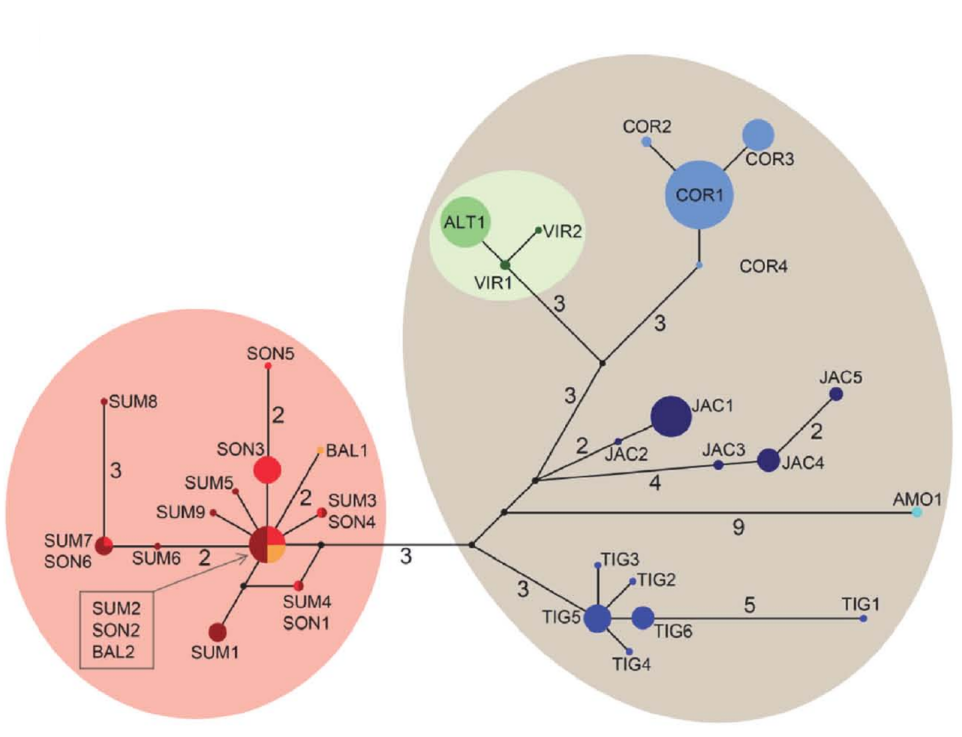
\includegraphics[width=\linewidth]{figures/tigers.png}
\caption{\scriptsize{Haplotype network of tigers\\
(Wilting et al. 2015)}}
\end{figure}
}
\only<3>{
\begin{figure}
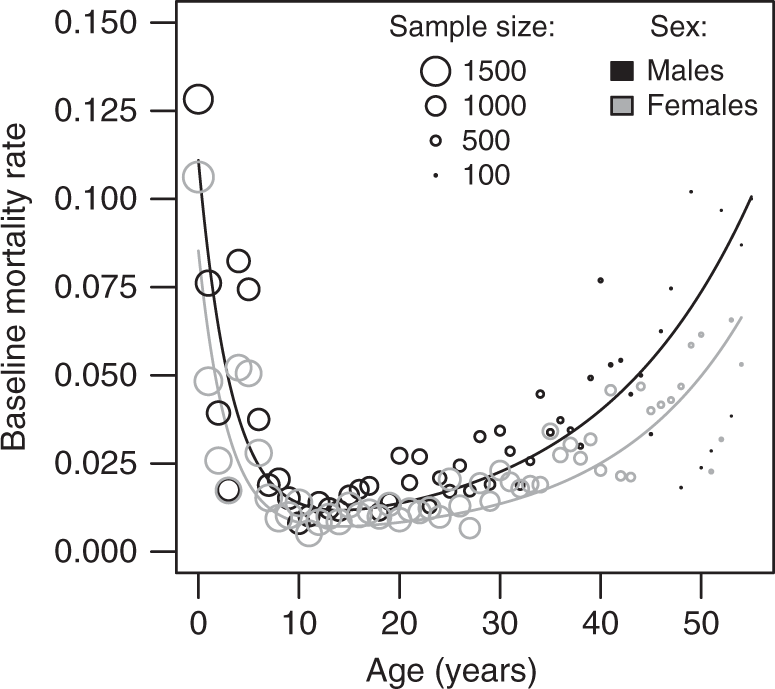
\includegraphics[width=\linewidth]{figures/eles_mortality.png}
\caption{\scriptsize{Yearly mortality rates of Myanmar timber elephants\\
(Lahdenperä et al. 2018)}}
\end{figure}
}
\only<4>{
\begin{figure}
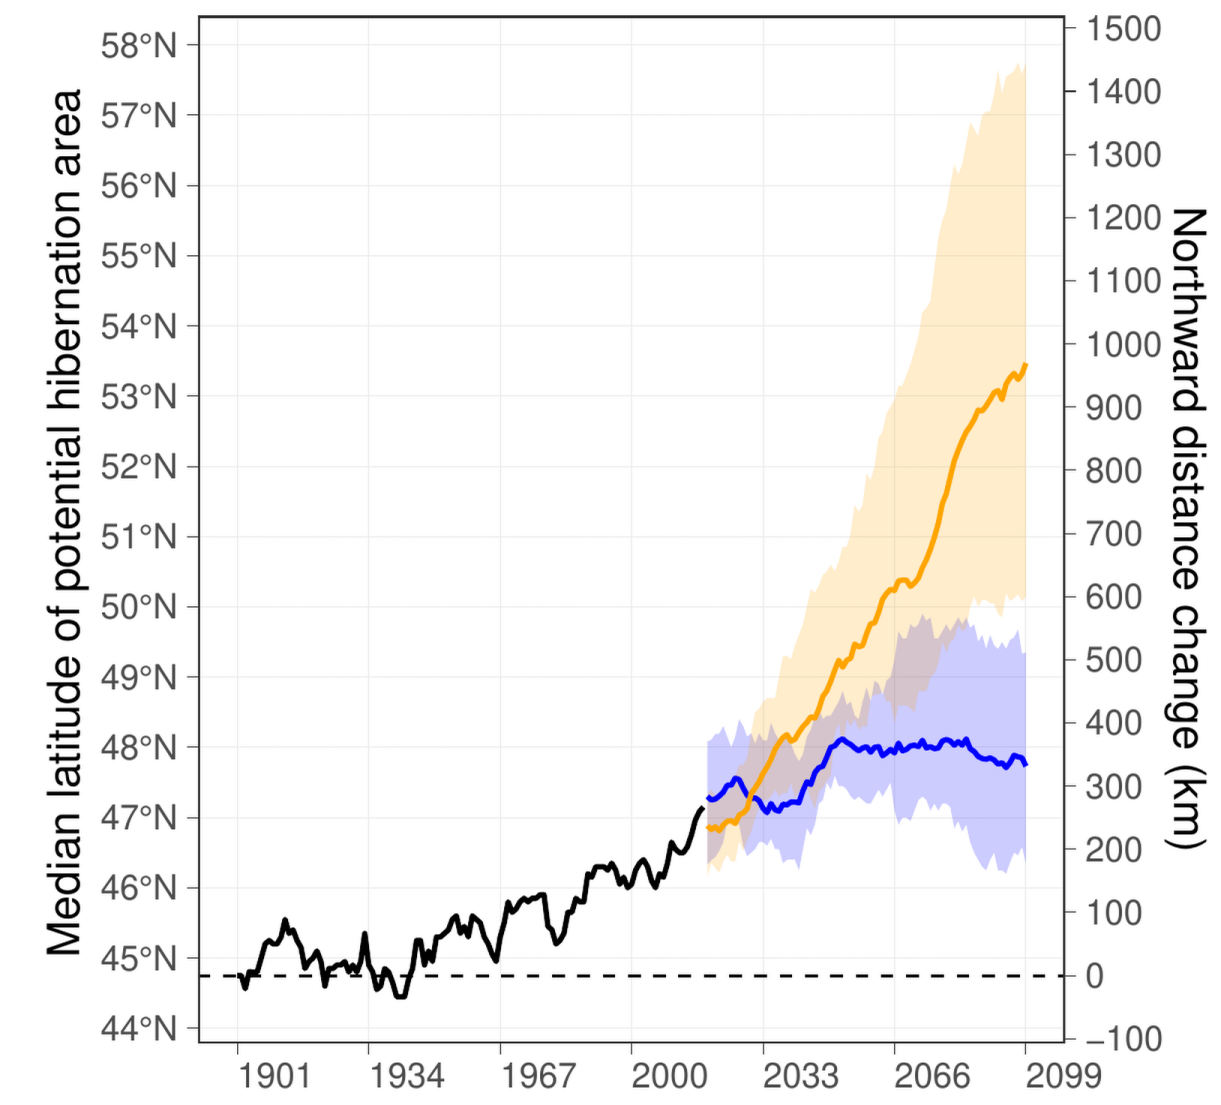
\includegraphics[width=\linewidth]{figures/bats_hibernation.png}
\caption{\scriptsize{Potential hibernation area of common noctule bats\\
(Kravchenko et al. 2025)}}
\end{figure}
}
\end{minipage}
}
\end{column}
\end{columns}

\uncover<6->{
\begin{callout}
\bluebold{Goals of statistics}
\begin{itemize}
\item mediates between a \blueit{sample} and the \blueit{population}
\item provides methods to draw as many conclusions as precisely as possible with as minimum \blueit{sampling effort} as possible
\end{itemize}
\end{callout}
}
\uncover<7>{
Some practical questions we will tackle:\

\emph{How \bluenorm{large} does the sample need to be? How to recognise and describe \bluenorm{relationships} among variables? How to quantify the \bluenorm{reliability} of the conclusions}?
}
\end{frame}

\begin{frame}{Population and sample --- definitions}
\protect\phantomsection\label{population-and-sample-definitions}
\bluebold{An adequate sample}

a statistical sample should adequately \bluenorm{represent} the
composition and properties of the entire population

\pause

\vspace{0.5cm}

\bluebold{The population}

this is the level at which you want to \bluenorm{discuss} your results

\pause

\(\rightarrow\) depends on the \bluenorm{research question}!

\pause

\vspace{0.5cm}

\textcolor{red}{Is a blood sample an adequate statistical sample?}

\vspace{1em}

\tightlist

\begin{itemize}[<+->]
\item
  Yes?
\item
  No?
\item
  \bluenorm{It depends!}
\end{itemize}
\end{frame}

\begin{frame}{Population and sample --- in practice}
\protect\phantomsection\label{population-and-sample-in-practice}
\textcolor{red}{Which design would you prefer to study a new drug aiming at preventing stroke?}

\footnotesize from \bluenorm{Ulrich Dirnagl} (Charité,
Berlin)\normalsize

\begin{columns}[T]
\begin{column}{0.45\linewidth}
\footnotesize

\begin{center}
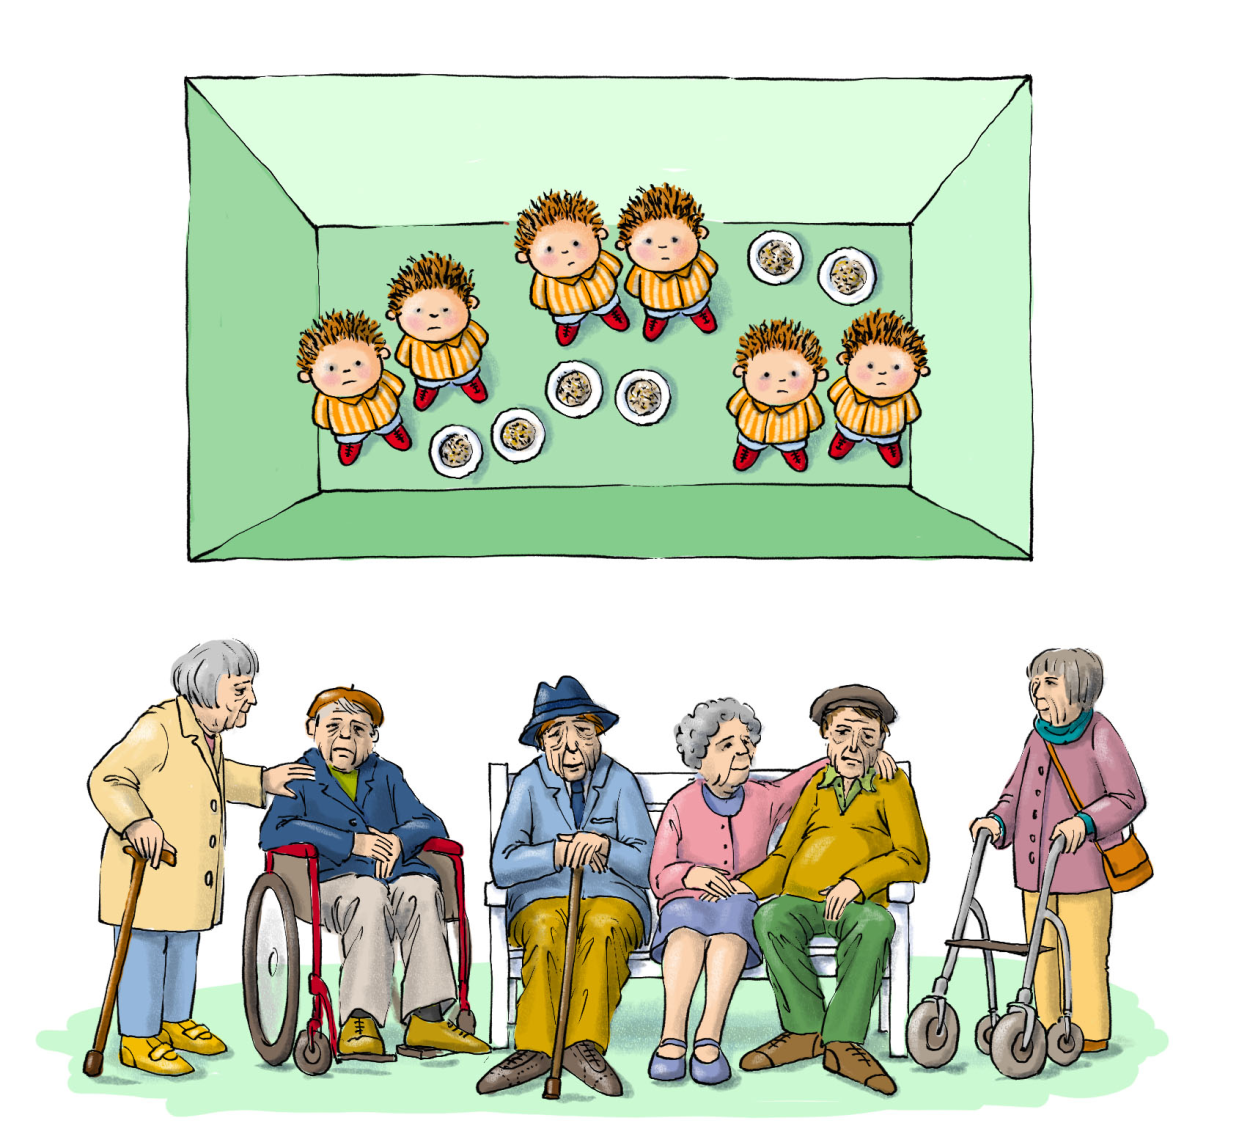
\includegraphics[width=\linewidth,height=4cm,keepaspectratio]{figures/twin_studies.png}
\end{center}

\normalsize
\end{column}

\begin{column}{0.55\linewidth}
\bluebold{DESIGN A}

healthy, pubertal male twins raised in 6 m\(^2\) isolator tents on an
enriched granola diet

\begin{center}
\textbf{vs.}
\end{center}

\bluebold{DESIGN B}

patients of both sexes, elderly, comorbid, multiple medications, exposed
to multiple pathogens and antigens throughout life
\end{column}
\end{columns}

\pause

\begin{callout}
\centering
The right \blueit{sampling design} may increase the external validity of your findings!
\end{callout}

\pause

\textcolor{red}{What would you mostly find in the medical literature?}
\end{frame}

\begin{frame}{Population and sample --- external validity}
\protect\phantomsection\label{population-and-sample-external-validity}
\footnotesize

\begin{center}
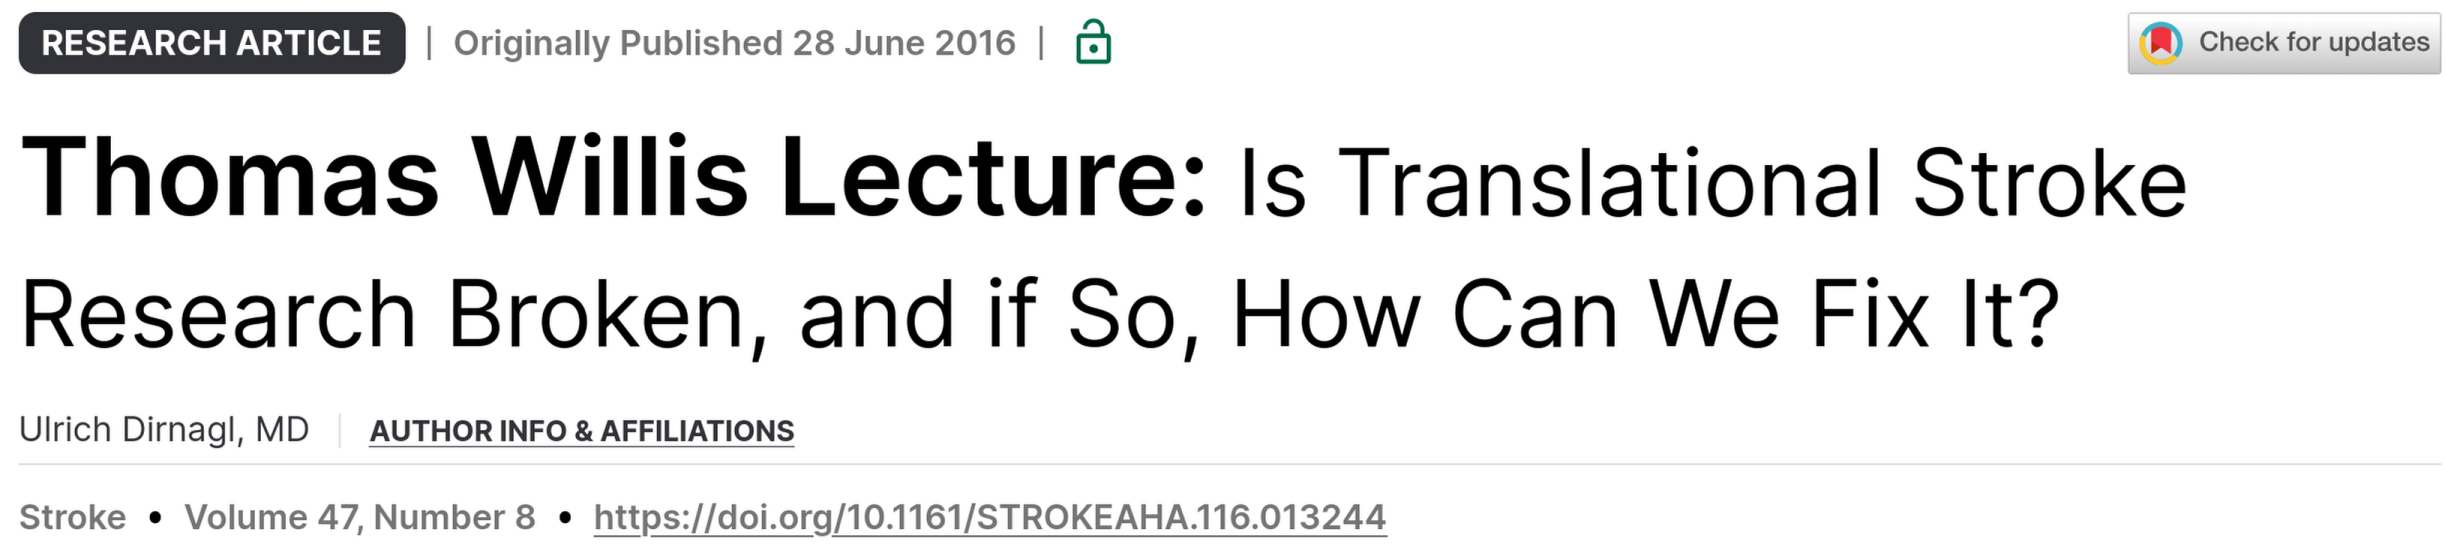
\includegraphics[width=\linewidth,height=3cm,keepaspectratio]{figures/twin_studies_title.png}
\end{center}

\normalsize

\vspace{0.3cm}

\scriptsize ``With few exceptions, stroke research is conducted in
healthy, very young, male inbred rodent strains raised under specific
pathogen-free conditions and fed a diet optimized for high fertility and
overall health. The equivalent human cohort would be healthy pubertal
twins raised in 6 m\(^2\) isolator tents on an enriched granola diet,
but patients with stroke are elderly, of both sexes, comorbid, on
multiple medications, and have had exposure to numerous pathogens and
antigens throughout their life. {[}\ldots{]} As a general rule, the
closer stroke models have mimicked patients with stroke {[}\ldots{]},
the more substantial has been the loss in efficacy of the treatment
effects.''

\footnotesize\bluebold{See also} Voelkl, B., Würbel, H., Krzywinski, M.
\emph{et al.} The standardization fallacy. \emph{Nat Methods}
\textbf{18}, 5--7 (2021).
\url{https://doi.org/10.1038/s41592-020-01036-9}\normalsize
\end{frame}

\begin{frame}{Population and sample --- sampling effort}
\protect\phantomsection\label{population-and-sample-sampling-effort}
The \blueit{sampling effort} should:

\begin{itemize}
\tightlist
\item
  maximise the \blueit{sample size}
\item
  minimise the \blueit{dependence} between objects
\item
  (given constraints: time, money, impact\ldots)
\end{itemize}

\pause

\vspace{0.5cm}

\textcolor{red}{Assuming that you only have a few minutes to sample hair in the classroom in order to estimate the average length of a piece of hair in the population, what should you do?}

\begin{enumerate}
\tightlist
\item
  sample 10,000 pieces of hair on 2 individuals?
\item
  sample 1,000 pieces of hair on 10 individuals?
\item
  sample 500 pieces of hair on 4 males \& 4 females?
\end{enumerate}

\pause

\vspace{0.5cm}

\(\rightarrow\) the best strategy depends on the extent to which hair
length depends on sex \& on the sex-ratio in \blueit{population}!
\end{frame}

\begin{frame}{Population and sample --- dependence between objects}
\protect\phantomsection\label{population-and-sample-dependence-between-objects}
\vspace{0.5cm}

\bluebold{Dependence between objects}

interrelationships between objects of the sample may lead to
similarities of properties or measurements to be analysed

\vspace{0.5cm}
\bluebold{Usual sources of dependence}

\begin{itemize}
\tightlist
\item
  time \(\rightarrow\) generates \blueit{temporal autocorrelation}
\item
  location \(\rightarrow\) generates \blueit{spatial autocorrelation}
\item
  measurements on the same individual \(\rightarrow\) generates
  \blueit{pseudoreplication}
\item
  pedigree/ancestry \(\rightarrow\) generates
  \blueit{genetic correlation}
\end{itemize}
\end{frame}

\begin{frame}{Population and sample --- dependence between objects}
\protect\phantomsection\label{population-and-sample-dependence-between-objects-1}
\bluebold{Scenario I} stress hormone concentrations in faeces of
\bluenorm{unknown} roe deer, sampled in southern Brandenburg and in the
proximity of an airport

\begin{columns}[T]
\begin{column}{0.5\linewidth}
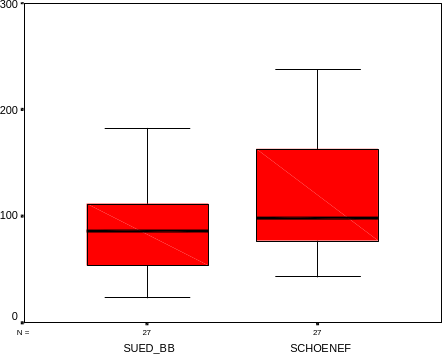
\includegraphics[width=0.95\linewidth,height=\textheight,keepaspectratio]{figures/deer_full.png}
\end{column}

\begin{column}{0.5\linewidth}
\vspace{1cm}

Mann-Whitney U-test\footnote<\value{beamerpauses}->[frame]{\footnotesize a
  non-parametric alternative to the unpaired t-test which is more robust}:\\
p = 0.079; n = 54

difference of means: 26.5

\pause

\vspace{0.3cm}

\bluebold{problem}\\
population = faeces \(\rightarrow\) \blueit{pseudoreplication!}
\end{column}
\end{columns}
\end{frame}

\begin{frame}{Population and sample --- dependence between objects}
\protect\phantomsection\label{population-and-sample-dependence-between-objects-2}
\bluebold{Scenario II} stress hormone concentrations in faeces assigned
to \bluenorm{known} roe deer individuals, sampled in southern
Brandenburg and in the proximity of an airport

\begin{columns}[T]
\begin{column}{0.5\linewidth}
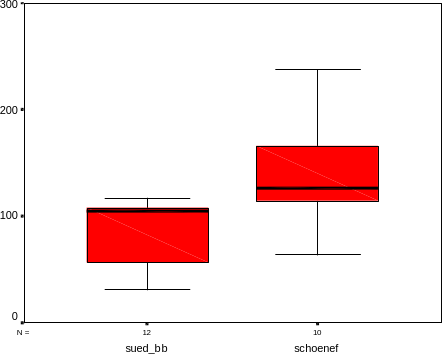
\includegraphics[width=0.95\linewidth,height=\textheight,keepaspectratio]{figures/deer_unique.png}
\end{column}

\begin{column}{0.5\linewidth}
\setcounter{footnote}{0}

\vspace{1cm}

Mann-Whitney U-test\footnote<\value{beamerpauses}->[frame]{\footnotesize a
  non-parametric alternative to the unpaired t-test which is more robust}:\\
p = 0.004; n = 22

difference of means: 48.8

\pause

\vspace{0.3cm}

\bluebold{solution}\\
population = deer

\begin{callout}
$\rightarrow$ fewer independent data points can contain more information than many dependent ones!
\end{callout}
\end{column}
\end{columns}
\end{frame}

\section{Random variables and probability
distributions}\label{random-variables-and-probability-distributions}

\begin{frame}{Random variables and probability distributions ---
definitions}
\protect\phantomsection\label{random-variables-and-probability-distributions-definitions}
\vspace{0.5cm}

\begin{itemize}
\item<1->{\bluebold{random variable} a variable which can take different values}
\item<2->{\bluebold{estimator} a method for estimating an unknown parameter using the sample-based measurements \\ 
$\rightarrow$ a random variable}
\item<3->{\bluebold{estimate} the estimation of the unknown parameter given by the estimator \\ 
$\rightarrow$ a realization from a random variable}
\end{itemize}

\vspace{1cm}

\uncover<4>{
\begin{callout}
Because they are computed from a sample rather than from the entire population, the estimator is a \blueit{random variable} and its outcome is called the \blueit{estimate}!
\end{callout}
}
\end{frame}

\begin{frame}{Random variables and probability distributions ---
definitions}
\protect\phantomsection\label{random-variables-and-probability-distributions-definitions-1}
To describe the outcome of a \blueit{random variable}, we use
\blueit{probability distributions}

\bluebold{Probability distributions}

\begin{itemize}
\tightlist
\item
  are compact and comprehensive description of the
  \blueit{relative frequency} of all possible values
\item
  comprises much more \blueit{information} than single estimator outcome
\item
  are the most important tool of the theory for statistical estimation
  and \blueit{tests}
\item
  serve as models for real data, which enables the estimation of
  \blueit{confidence intervals} and statistical \blueit{tests}
\end{itemize}

\begin{columns}[T]
\begin{column}{0.33\linewidth}
\footnotesize

\begin{figure}[H]

{\centering \includegraphics[width=\linewidth,height=2.3cm,keepaspectratio]{fundamentals_files/figure-beamer/unnamed-chunk-3-1.pdf}

}

\caption{\scriptsize normal distribution}

\end{figure}%

\normalsize
\end{column}

\begin{column}{0.33\linewidth}
\footnotesize

\begin{figure}[H]

{\centering \includegraphics[width=\linewidth,height=2.3cm,keepaspectratio]{fundamentals_files/figure-beamer/unnamed-chunk-4-1.pdf}

}

\caption{\scriptsize chi-squared distribution}

\end{figure}%

\normalsize
\end{column}

\begin{column}{0.33\linewidth}
\footnotesize

\begin{figure}[H]

{\centering \includegraphics[width=\linewidth,height=2.3cm,keepaspectratio]{fundamentals_files/figure-beamer/unnamed-chunk-5-1.pdf}

}

\caption{\scriptsize Poisson distribution}

\end{figure}%

\normalsize
\end{column}
\end{columns}
\end{frame}

\begin{frame}[fragile]{Random variables and probability distributions
--- empirical description}
\protect\phantomsection\label{random-variables-and-probability-distributions-empirical-description}
\bluebold{Qualitative data}

\begin{itemize}
\tightlist
\item
  observations (``measurements'') described by 2 or more
  \blueit{categories}
\item
  special case: \blueit{binary} data (2 categories)
\end{itemize}

\(\rightarrow\) can be fully described by a \blueit{contingency table},
i.e.~a table providing the number of observation for each category

\pause

\vspace{1em}

\begin{columns}[T]
\begin{column}{0.5\linewidth}
\centering\bluebold{tidyverse}

\footnotesize

\begin{Shaded}
\begin{Highlighting}[]
\NormalTok{iris }\SpecialCharTok{|\textgreater{}} \FunctionTok{count}\NormalTok{(Species)}
\end{Highlighting}
\end{Shaded}

\begin{verbatim}
     Species  n
1     setosa 50
2 versicolor 50
3  virginica 50
\end{verbatim}

\normalsize
\end{column}

\begin{column}{0.5\linewidth}
\centering\bluebold{base R}

\footnotesize

\begin{Shaded}
\begin{Highlighting}[]
\FunctionTok{table}\NormalTok{(iris}\SpecialCharTok{$}\NormalTok{Species)}
\end{Highlighting}
\end{Shaded}

\begin{verbatim}

    setosa versicolor  virginica 
        50         50         50 
\end{verbatim}

\normalsize
\end{column}
\end{columns}
\end{frame}

\begin{frame}[fragile]{Random variables and probability distributions
--- empirical description}
\protect\phantomsection\label{random-variables-and-probability-distributions-empirical-description-1}
\bluebold{Qualitative data}

\begin{itemize}
\tightlist
\item
  observations (``measurements'') described by 2 or more
  \blueit{categories}
\item
  special case: \blueit{binary} data (2 categories)
\end{itemize}

\(\rightarrow\) can be fully described by a \blueit{barplot}
illustrating the contingency table

\vspace{1em}

\begin{columns}[T]
\begin{column}{0.5\linewidth}
\footnotesize

\begin{Shaded}
\begin{Highlighting}[]
\FunctionTok{ggplot}\NormalTok{(iris) }\SpecialCharTok{+}
  \FunctionTok{aes}\NormalTok{(}\AttributeTok{x =}\NormalTok{ Species) }\SpecialCharTok{+}
  \FunctionTok{geom\_bar}\NormalTok{()}
\end{Highlighting}
\end{Shaded}

\normalsize
\end{column}

\begin{column}{0.5\linewidth}
\footnotesize

\begin{center}
\includegraphics[width=\linewidth,height=3cm,keepaspectratio]{fundamentals_files/figure-beamer/unnamed-chunk-9-1.pdf}
\end{center}

\normalsize
\end{column}
\end{columns}
\end{frame}

\begin{frame}[fragile]{Random variables and probability distributions
--- empirical description}
\protect\phantomsection\label{random-variables-and-probability-distributions-empirical-description-2}
\bluebold{Quantitative data}

\begin{itemize}
\tightlist
\item
  measurements (\blueit{continuous}) and counts (\blueit{discrete})
\item
  distance between each pair of data points is meaningful
\end{itemize}

\(\rightarrow\) can be fully described by an
\blueit{empirical cumulative distribution function} (ecdf)

\vspace{1em}

\begin{columns}[T]
\begin{column}{0.6\linewidth}
\footnotesize

\begin{Shaded}
\begin{Highlighting}[]
\FunctionTok{ggplot}\NormalTok{(iris) }\SpecialCharTok{+}
  \FunctionTok{aes}\NormalTok{(}\AttributeTok{x =}\NormalTok{ Petal.Length) }\SpecialCharTok{+}
  \FunctionTok{geom\_step}\NormalTok{(}\AttributeTok{stat =} \StringTok{"ecdf"}\NormalTok{) }\SpecialCharTok{+}
  \FunctionTok{geom\_point}\NormalTok{(}\AttributeTok{stat =} \StringTok{"ecdf"}\NormalTok{) }\SpecialCharTok{+}
  \FunctionTok{labs}\NormalTok{(}\AttributeTok{y =} \StringTok{"Cumulative probability"}\NormalTok{,}
       \AttributeTok{x =} \StringTok{"Petal length"}\NormalTok{)}
\end{Highlighting}
\end{Shaded}

\normalsize
\end{column}

\begin{column}{0.4\linewidth}
\footnotesize

\begin{center}
\includegraphics[width=\linewidth,height=3cm,keepaspectratio]{fundamentals_files/figure-beamer/unnamed-chunk-11-1.pdf}
\end{center}

\normalsize
\end{column}
\end{columns}
\end{frame}

\begin{frame}[fragile]{Random variables and probability distributions
--- empirical description}
\protect\phantomsection\label{random-variables-and-probability-distributions-empirical-description-3}
\bluebold{Quantiles}

\begin{itemize}
\tightlist
\item
  the ecdf directly provides \blueit{quantiles}, i.e.~the values at or
  below which given \blueit{proportions} of the data fall
\end{itemize}

\begin{columns}[T]
\begin{column}{0.6\linewidth}
\footnotesize

\begin{Shaded}
\begin{Highlighting}[]
\FunctionTok{quantile}\NormalTok{(iris}\SpecialCharTok{$}\NormalTok{Petal.Length, }\AttributeTok{probs =} \FloatTok{0.75}\NormalTok{)}
\end{Highlighting}
\end{Shaded}

\begin{verbatim}
75% 
5.1 
\end{verbatim}

\normalsize
\end{column}

\begin{column}{0.4\linewidth}
\footnotesize

\begin{center}
\includegraphics[width=\linewidth,height=3cm,keepaspectratio]{fundamentals_files/figure-beamer/unnamed-chunk-13-1.pdf}
\end{center}

\normalsize
\end{column}
\end{columns}

\textbf{NB:}

\begin{itemize}
\tightlist
\item
  reading up from a given cumulative probability (e.g.~\bluenorm{0.75})
  to the curve, then across to the x-axis, identifies the corresponding
  \blueit{quantile} of petal length
\end{itemize}
\end{frame}

\begin{frame}[fragile]{Random variables and probability distributions
--- comparing distributions}
\protect\phantomsection\label{random-variables-and-probability-distributions-comparing-distributions}
\bluebold{Quantile–quantile plot}

\begin{itemize}
\tightlist
\item
  the QQ plot compares 2 distributions by plotting their quantiles
  against each other
\item
  it is often used to compare a distribution derived from the data to a
  normal distribution with same mean and variance (default in
  e.g.~\texttt{geom\_qq()})
\end{itemize}

\begin{columns}[T]
\begin{column}{0.6\linewidth}
\footnotesize

\begin{Shaded}
\begin{Highlighting}[]
\FunctionTok{set.seed}\NormalTok{(}\DecValTok{123}\NormalTok{) }\CommentTok{\# randomness is "fixed"}
\FunctionTok{tibble}\NormalTok{(}\AttributeTok{x =} \FunctionTok{rnorm}\NormalTok{(}\AttributeTok{n =} \DecValTok{50}\NormalTok{)) }\SpecialCharTok{|\textgreater{}} \CommentTok{\# normal}
\FunctionTok{ggplot}\NormalTok{(}\FunctionTok{aes}\NormalTok{(}\AttributeTok{sample =}\NormalTok{ x)) }\SpecialCharTok{+}
  \FunctionTok{geom\_qq}\NormalTok{(}\AttributeTok{shape =} \DecValTok{1}\NormalTok{) }\SpecialCharTok{+}
  \FunctionTok{geom\_qq\_line}\NormalTok{()}
\end{Highlighting}
\end{Shaded}

\normalsize
\end{column}

\begin{column}{0.4\linewidth}
\footnotesize

\begin{center}
\includegraphics[width=\linewidth,height=2.5cm,keepaspectratio]{fundamentals_files/figure-beamer/unnamed-chunk-15-1.pdf}
\end{center}

\normalsize
\end{column}
\end{columns}

\pause

\begin{itemize}
\tightlist
\item
  if the points fall \bluenorm{close to the QQ line}, they are
  \bluenorm{compatible} with expectations under a
  \blueit{normal distribution}
\end{itemize}

\footnotesize

\normalsize
\end{frame}

\begin{frame}[fragile]{Random variables and probability distributions
--- comparing distributions}
\protect\phantomsection\label{random-variables-and-probability-distributions-comparing-distributions-1}
\bluebold{Quantile–quantile plot}

\begin{itemize}
\tightlist
\item
  the QQ plot compares 2 distributions by plotting their quantiles
  against each other
\item
  it is often used to compare a distribution derived from the data to a
  normal distribution with same mean and variance (default in
  e.g.~\texttt{geom\_qq()})
\end{itemize}

\begin{columns}[T]
\begin{column}{0.6\linewidth}
\footnotesize

\begin{Shaded}
\begin{Highlighting}[]
\FunctionTok{set.seed}\NormalTok{(}\DecValTok{123}\NormalTok{) }\CommentTok{\# randomness is "fixed"}
\FunctionTok{tibble}\NormalTok{(}\AttributeTok{x =} \FunctionTok{rchisq}\NormalTok{(}\AttributeTok{n =} \DecValTok{50}\NormalTok{, }\AttributeTok{df =} \DecValTok{2}\NormalTok{)) }\SpecialCharTok{|\textgreater{}} \CommentTok{\# chi{-}squared}
\FunctionTok{ggplot}\NormalTok{(}\FunctionTok{aes}\NormalTok{(}\AttributeTok{sample =}\NormalTok{ x)) }\SpecialCharTok{+}
  \FunctionTok{geom\_qq}\NormalTok{(}\AttributeTok{shape =} \DecValTok{1}\NormalTok{) }\SpecialCharTok{+}
  \FunctionTok{geom\_qq\_line}\NormalTok{()}
\end{Highlighting}
\end{Shaded}

\normalsize
\end{column}

\begin{column}{0.4\linewidth}
\footnotesize

\begin{center}
\includegraphics[width=\linewidth,height=2.5cm,keepaspectratio]{fundamentals_files/figure-beamer/unnamed-chunk-17-1.pdf}
\end{center}

\normalsize
\end{column}
\end{columns}

\begin{itemize}
\tightlist
\item
  if the points fall \bluenorm{close to the QQ line}, they are
  \bluenorm{compatible} with expectations under a
  \blueit{normal distribution}
\item
  if many of the points fall \bluenorm{far from the QQ line}, they are
  not \bluenorm{compatible} with expectations under a
  \blueit{normal distribution} (see next course)
\end{itemize}
\end{frame}

\begin{frame}[fragile]{Random variables and probability distributions
--- comparing distributions}
\protect\phantomsection\label{random-variables-and-probability-distributions-comparing-distributions-2}
\bluebold{Quantitative data}

a \blueit{histogram} does \textcolor{red}{NOT} fully describe a
distribution

\begin{columns}[T]
\begin{column}{0.6\linewidth}
\footnotesize

\begin{Shaded}
\begin{Highlighting}[]
\FunctionTok{ggplot}\NormalTok{(iris) }\SpecialCharTok{+}
  \FunctionTok{aes}\NormalTok{(}\AttributeTok{x =}\NormalTok{ Petal.Length) }\SpecialCharTok{+}
  \FunctionTok{geom\_histogram}\NormalTok{(}\AttributeTok{colour =} \StringTok{"white"}\NormalTok{) }\SpecialCharTok{+}
  \FunctionTok{geom\_rug}\NormalTok{()}
\end{Highlighting}
\end{Shaded}

\normalsize
\end{column}

\begin{column}{0.4\linewidth}
\footnotesize

\begin{center}
\includegraphics[width=\linewidth,height=3cm,keepaspectratio]{fundamentals_files/figure-beamer/unnamed-chunk-19-1.pdf}
\end{center}

\normalsize
\end{column}
\end{columns}
\end{frame}

\begin{frame}[fragile]{Random variables and probability distributions
--- comparing distributions}
\protect\phantomsection\label{random-variables-and-probability-distributions-comparing-distributions-3}
\bluebold{Quantitative data}

a \blueit{histogram} does \textcolor{red}{NOT} fully describe a
distribution

\begin{columns}[T]
\begin{column}{0.6\linewidth}
\footnotesize

\begin{Shaded}
\begin{Highlighting}[]
\FunctionTok{ggplot}\NormalTok{(iris) }\SpecialCharTok{+}
  \FunctionTok{aes}\NormalTok{(}\AttributeTok{x =}\NormalTok{ Petal.Length) }\SpecialCharTok{+}
  \FunctionTok{geom\_histogram}\NormalTok{(}\AttributeTok{colour =} \StringTok{"white"}\NormalTok{, }\AttributeTok{binwidth =} \FloatTok{0.5}\NormalTok{) }\SpecialCharTok{+}
  \FunctionTok{geom\_rug}\NormalTok{()}
\end{Highlighting}
\end{Shaded}

\normalsize
\end{column}

\begin{column}{0.4\linewidth}
\footnotesize

\begin{center}
\includegraphics[width=\linewidth,height=3cm,keepaspectratio]{fundamentals_files/figure-beamer/unnamed-chunk-21-1.pdf}
\end{center}

\normalsize
\end{column}
\end{columns}

\textbf{NB:}

\begin{itemize}
\tightlist
\item
  the choice of bin width changes the perceived shape of the
  distribution\\
  \(\rightarrow\) there is no single ``correct'' histogram for a given
  dataset
\item
  not the best tool to check for normality (use Q-Q plots instead)
\end{itemize}
\end{frame}

\begin{frame}{Random variables and probability distributions ---
theoretical distributions}
\protect\phantomsection\label{random-variables-and-probability-distributions-theoretical-distributions}
\footnotesize

\begin{center}
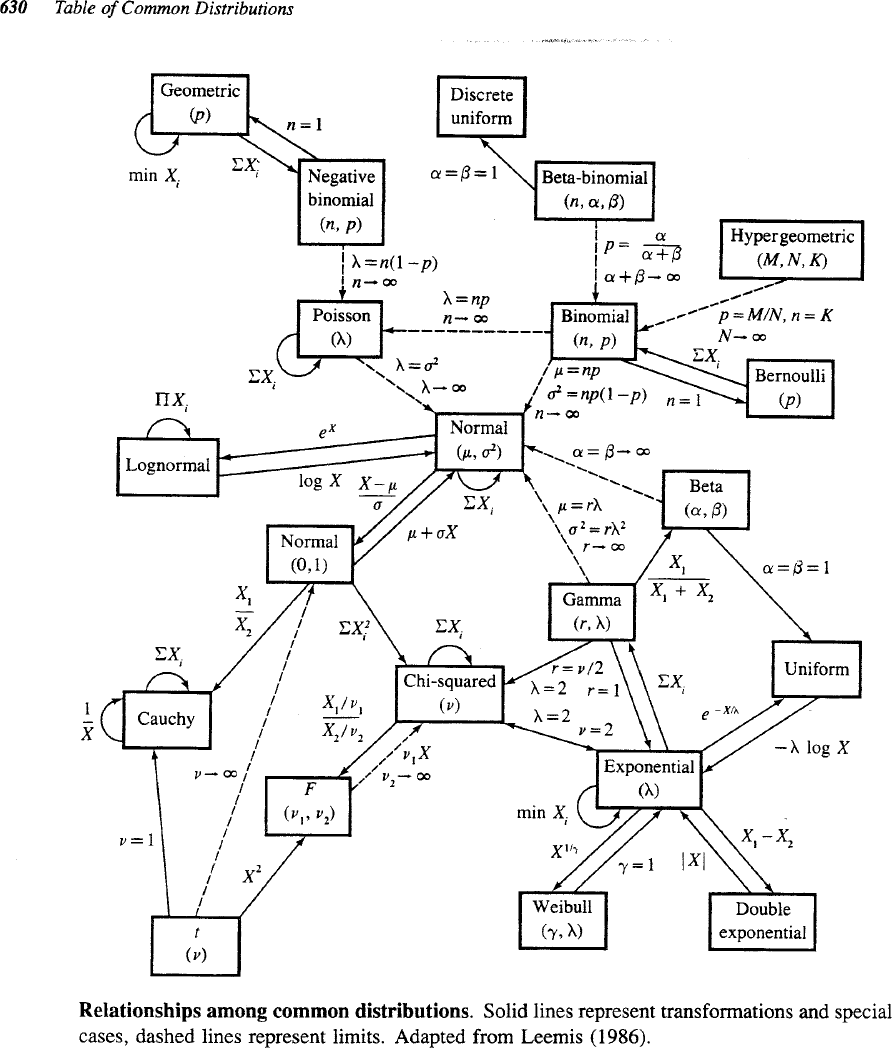
\includegraphics[width=\linewidth,height=7cm,keepaspectratio]{figures/distributions.png}
\end{center}

\normalsize

\centering \footnotesize from Casella \& Berger
\emph{Statistical Inference}, 1990\normalsize
\end{frame}

\begin{frame}[fragile]{Random variables and probability distributions
--- the binomial distribution}
\protect\phantomsection\label{random-variables-and-probability-distributions-the-binomial-distribution}
\blueit{Probability density function} (aka \emph{pdf}) for a probability
of success of 0.2, over 10 trials:

\footnotesize

\begin{Shaded}
\begin{Highlighting}[]
\FunctionTok{dbinom}\NormalTok{(}\AttributeTok{x =} \DecValTok{0}\SpecialCharTok{:}\DecValTok{10}\NormalTok{, }\AttributeTok{size =} \DecValTok{10}\NormalTok{, }\AttributeTok{prob =} \FloatTok{0.2}\NormalTok{)}
\end{Highlighting}
\end{Shaded}

\normalsize

\begin{columns}[T]
\begin{column}{0.55\linewidth}
\footnotesize

\begin{center}
\includegraphics[width=\linewidth,height=4cm,keepaspectratio]{fundamentals_files/figure-beamer/unnamed-chunk-24-1.pdf}
\end{center}

\normalsize
\end{column}

\begin{column}{0.45\linewidth}
\begin{center}
$f(x,n,p) = \Pr(X=x) = \dbinom{n}{x}p^x(1-p)^{n-x}$

\vspace{4pt}
{\footnotesize for $x = 0, 1, 2, \ldots, n$, where}
\vspace{4pt}

$\dbinom{n}{x} = \dfrac{n!}{x!(n-x)!}$
\end{center}
\end{column}
\end{columns}

\onslide*<1>{
The density gives the expected probability for exactly \textbf{\emph{x}} successes in \textbf{\emph{n}} \blueit{independent} binary trials if the probability for one success is equal to \textbf{\emph{p}}
}
\onslide*<2>{
If the probability of catching a bird in one attempt is now expected to be 5\%. Then, \textcolor{red}{what is the chance that the biologist will capture exactly one bird in 10 attempts?}
}
\end{frame}

\begin{frame}[fragile]{Random variables and probability distributions
--- the binomial distribution}
\protect\phantomsection\label{random-variables-and-probability-distributions-the-binomial-distribution-1}
\blueit{Density} for exactly one \blueit{success}, for a probability of
success of 0.05 over 10 trials:

\footnotesize

\begin{Shaded}
\begin{Highlighting}[]
\FunctionTok{dbinom}\NormalTok{(}\AttributeTok{x =} \DecValTok{1}\NormalTok{, }\AttributeTok{size =} \DecValTok{10}\NormalTok{, }\AttributeTok{prob =} \FloatTok{0.05}\NormalTok{)}
\end{Highlighting}
\end{Shaded}

\normalsize

\begin{columns}[T]
\begin{column}{0.55\linewidth}
\footnotesize

\begin{center}
\includegraphics[width=\linewidth,height=4cm,keepaspectratio]{fundamentals_files/figure-beamer/unnamed-chunk-26-1.pdf}
\end{center}

\normalsize
\end{column}

\begin{column}{0.45\linewidth}
\begin{center}
$f(x,n,p) = \Pr(X=x) = \dbinom{n}{x}p^x(1-p)^{n-x}$

\vspace{4pt}
{\footnotesize for $x = 0, 1, 2, \ldots, n$, where}
\vspace{4pt}

$\dbinom{n}{x} = \dfrac{n!}{x!(n-x)!}$
\end{center}
\end{column}
\end{columns}

\onslide*<1>{
If the probability of catching a bird in one attempt is now expected to be 5\%. Then, \textcolor{red}{what is the chance that the biologist will capture exactly one bird in 10 attempts?}
}
\end{frame}

\begin{frame}[fragile]{Random variables and probability distributions
--- the binomial distribution}
\protect\phantomsection\label{random-variables-and-probability-distributions-the-binomial-distribution-2}
\blueit{Cumulative distribution function} (\emph{cdf}) for a probability
of success of 0.2 over 10 trials:

\footnotesize

\begin{Shaded}
\begin{Highlighting}[]
\FunctionTok{pbinom}\NormalTok{(}\AttributeTok{q =} \DecValTok{0}\SpecialCharTok{:}\DecValTok{10}\NormalTok{, }\AttributeTok{size =} \DecValTok{10}\NormalTok{, }\AttributeTok{prob =} \FloatTok{0.2}\NormalTok{)}
\end{Highlighting}
\end{Shaded}

\normalsize

\begin{columns}[T]
\begin{column}{0.55\linewidth}
\footnotesize

\begin{center}
\includegraphics[width=\linewidth,height=4cm,keepaspectratio]{fundamentals_files/figure-beamer/unnamed-chunk-28-1.pdf}
\end{center}

\normalsize
\end{column}

\begin{column}{0.45\linewidth}
\begin{center}
$F(x,n,p) = \Pr(X \le x) = \displaystyle\sum_{i=0}^{\lfloor x \rfloor} \dbinom{n}{i}p^i(1-p)^{n-i}$

\vspace{4pt}
{\footnotesize where $\dbinom{n}{i} = \dfrac{n!}{i!(n-i)!}$}
\end{center}
\end{column}
\end{columns}

\onslide*<1>{
The cumulative probability gives the expected probability for \textbf{\emph{x}} or fewer successes in \textbf{\emph{n}} \blueit{independent} binary trials if the probability for one success is equal to \textbf{\emph{p}}
}
\onslide*<2>{
If the probability of catching a bird in one attempt is expected to be 5\%. Then,\\
\textcolor{red}{what is the chance that the biologist will capture at least two birds in 10 attempts?}
}
\end{frame}

\begin{frame}[fragile]{Random variables and probability distributions
--- the binomial distribution}
\protect\phantomsection\label{random-variables-and-probability-distributions-the-binomial-distribution-3}
Probability of at least 2 successes for a probability of success of 0.05
over 10 trials:

\footnotesize

\begin{Shaded}
\begin{Highlighting}[]
\DecValTok{1} \SpecialCharTok{{-}} \FunctionTok{pbinom}\NormalTok{(}\AttributeTok{q =} \DecValTok{1}\NormalTok{, }\AttributeTok{size =} \DecValTok{10}\NormalTok{, }\AttributeTok{prob =} \FloatTok{0.05}\NormalTok{)}
\end{Highlighting}
\end{Shaded}

\normalsize

\begin{columns}[T]
\begin{column}{0.55\linewidth}
\footnotesize

\begin{center}
\includegraphics[width=\linewidth,height=4cm,keepaspectratio]{fundamentals_files/figure-beamer/unnamed-chunk-30-1.pdf}
\end{center}

\normalsize
\end{column}

\begin{column}{0.45\linewidth}
\begin{center}
$F(x,n,p) = \Pr(X \le x) = \displaystyle\sum_{i=0}^{\lfloor x \rfloor} \dbinom{n}{i}p^i(1-p)^{n-i}$

\vspace{4pt}
{\footnotesize where $\dbinom{n}{i} = \dfrac{n!}{i!(n-i)!}$}
\end{center}
\end{column}
\end{columns}

\onslide*<1>{
If the probability of catching a bird in one attempt is expected to be 5\%. Then,\\
\textcolor{red}{what is the chance that the biologist will capture at least two birds in 10 attempts?}
}
\end{frame}

\begin{frame}[fragile]{Random variables and probability distributions
--- the normal distribution}
\protect\phantomsection\label{random-variables-and-probability-distributions-the-normal-distribution}
\blueit{Probability density function} for a mean of 0 and a standard
deviation of 1\\
(i.e.~the standard normal distribution)

\footnotesize

\begin{Shaded}
\begin{Highlighting}[]
\FunctionTok{dnorm}\NormalTok{(}\AttributeTok{x =} \FunctionTok{seq}\NormalTok{(}\SpecialCharTok{{-}}\DecValTok{4}\NormalTok{, }\DecValTok{4}\NormalTok{, }\AttributeTok{length.out =} \DecValTok{100}\NormalTok{))}
\end{Highlighting}
\end{Shaded}

\normalsize

\begin{columns}[T]
\begin{column}{0.6\linewidth}
\footnotesize

\begin{center}
\includegraphics[width=\linewidth,height=4cm,keepaspectratio]{fundamentals_files/figure-beamer/unnamed-chunk-32-1.pdf}
\end{center}

\normalsize
\end{column}

\begin{column}{0.4\linewidth}
\vspace{0.5cm}

standard normal distribution

\begin{center}
$f(x) = \dfrac{1}{\sqrt{2\pi}}\, e^{-x^2/2}$
\end{center}

\vspace{1cm}

general normal distribution

\begin{center}
$f(x,\mu,\sigma) = \dfrac{1}{\sigma\sqrt{2\pi}}\, e^{-\frac{(x-\mu)^2}{2\sigma^2}}$
\end{center}
\end{column}
\end{columns}

\textbf{NB:} it can be parametrised with mean (\(\mu\)) and either the
SD (\(\sigma\)) or the variance (\(\sigma^2\)), with
\(\hat{\sigma^2} = \frac{1}{n - 1} \sum_{i=1}^n \left(x_i - \hat{\mu}\right)^2\)
(note that the '' \(\hat{}\) '' refers to estimates from data, as
opposed to population values)
\end{frame}

\begin{frame}{Random variables and probability distributions --- the
normal distribution}
\protect\phantomsection\label{random-variables-and-probability-distributions-the-normal-distribution-1}
\bluebold{From general to standard}: the \blueit{z-scores}
transformation

if \(X \sim \mathcal{N}(\mu, \sigma)\), then

\(z = \frac{x-\hat{\mu}}{\hat{\sigma}} \sim \mathcal{N}(0, 1)\)

\pause

\bluebold{Back to general}

if \(Z \sim \mathcal{N}(0, 1)\), then given \(\hat{\mu}\) and
\(\hat{\sigma}\), we can revert the z-scores transformation:

\(x = (z \times \hat{\sigma}) + \hat{\mu}\)

\pause

\begin{itemize}
\tightlist
\item
  the z-scores transformation is often used within statistical tests
\item
  it can also help to understand how extreme some measurements are when
  units are not familiar (e.g.~\(z = 3\) correspond to a value 3 SD
  above the mean)
\item
  outliers are often identified as observations with absolute z-scores
  \textgreater{} 3 or 4, but very large outliers can inflate
  \(\hat{\sigma}\) and thus be masked; in any case
  \bluenorm{do not ditch outliers without discussing it!}
\end{itemize}
\end{frame}

\begin{frame}[fragile]{Random variables and probability distributions
--- the normal distribution}
\protect\phantomsection\label{random-variables-and-probability-distributions-the-normal-distribution-2}
\blueit{Cumulative distribution function} for a mean of 0 and a standard
deviation of 1\\
(i.e.~the standard normal distribution)

\begin{columns}[T]
\begin{column}{0.6\linewidth}
\footnotesize

\begin{Shaded}
\begin{Highlighting}[]
 \FunctionTok{pnorm}\NormalTok{(}\AttributeTok{q =} \FunctionTok{seq}\NormalTok{(}\SpecialCharTok{{-}}\DecValTok{4}\NormalTok{, }\DecValTok{4}\NormalTok{, }\AttributeTok{length.out =} \DecValTok{100}\NormalTok{))}
\end{Highlighting}
\end{Shaded}

\normalsize

\footnotesize

\begin{center}
\includegraphics[width=\linewidth,height=4cm,keepaspectratio]{fundamentals_files/figure-beamer/unnamed-chunk-34-1.pdf}
\end{center}

\normalsize
\end{column}

\begin{column}{0.4\linewidth}
standard normal distribution

\begin{center}
$F(x) = \Pr(X \le x) = \displaystyle\int_{-\infty}^{x} \dfrac{1}{\sqrt{2\pi}}\, e^{-t^2/2}\, dt$
\end{center}

\vspace{1cm}

general normal distribution

\begin{center}
$F(x,\mu,\sigma) = \Pr(X \le x) = \displaystyle\int_{-\infty}^{x} \dfrac{1}{\sigma\sqrt{2\pi}}\, e^{-\frac{(t-\mu)^2}{2\sigma^2}}\, dt$
\end{center}
\end{column}
\end{columns}
\end{frame}

\begin{frame}{Random variables and probability distributions --- the
normal distribution}
\protect\phantomsection\label{random-variables-and-probability-distributions-the-normal-distribution-3}
\textcolor{red}{What is the expected probability that an outcome \emph{x} will be between -1.96 and +1.96 if this event is the result of a standard normal distribution?}

\vspace{1em}

\begin{columns}[T]
\begin{column}{0.5\linewidth}
\footnotesize

\begin{center}
\includegraphics[width=\linewidth,height=4cm,keepaspectratio]{fundamentals_files/figure-beamer/unnamed-chunk-35-1.pdf}
\end{center}

\normalsize
\end{column}

\pause

\begin{column}{0.5\linewidth}
\footnotesize

\begin{center}
\includegraphics[width=\linewidth,height=4cm,keepaspectratio]{fundamentals_files/figure-beamer/unnamed-chunk-36-1.pdf}
\end{center}

\normalsize
\end{column}
\end{columns}
\end{frame}

\begin{frame}{Random variables and probability distributions --- the
normal distribution}
\protect\phantomsection\label{random-variables-and-probability-distributions-the-normal-distribution-4}
\textcolor{red}{What is the probability for an observation following a normal distribution to have a value more extreme than:}

\begin{itemize}
\tightlist
\item
  \textcolor{red}{one SD?}
\item
  \textcolor{red}{two SD?}
\item
  \textcolor{red}{three SD?}
\end{itemize}

\bluebold{Instructions}

\begin{itemize}
\tightlist
\item
  fix the mean to 0 and the SD to 1 to do the computation
\item
  then, try doing the same with a different mean and SD
\end{itemize}
\end{frame}

\begin{frame}{Random variables and probability distributions --- the
normal distribution}
\protect\phantomsection\label{random-variables-and-probability-distributions-the-normal-distribution-5}
\bluebold{Reverted situation}

\textcolor{red}{If random numbers are drawn from a standard normal distribution, where will the 75\% of central observations fall?}

\(\rightarrow\) the answer is given by the \blueit{quantile function}

\footnotesize

\begin{center}
\includegraphics[width=\linewidth,height=4cm,keepaspectratio]{fundamentals_files/figure-beamer/unnamed-chunk-37-1.pdf}
\end{center}

\normalsize
\end{frame}

\begin{frame}[fragile]{Random variables and probability distributions
--- summary}
\protect\phantomsection\label{random-variables-and-probability-distributions-summary}
\begin{columns}[T]
\begin{column}{0.31\linewidth}
\centering \texttt{dnorm(x\ =\ ...)}

\footnotesize

\begin{figure}[H]

{\centering \includegraphics[width=\linewidth,height=3cm,keepaspectratio]{fundamentals_files/figure-beamer/unnamed-chunk-38-1.pdf}

}

\caption{Probability density function}

\end{figure}%

\normalsize
\end{column}

\begin{column}{0.38\linewidth}
\centering \texttt{pnorm(q\ =\ ...)}

\footnotesize

\begin{figure}[H]

{\centering \includegraphics[width=\linewidth,height=3cm,keepaspectratio]{fundamentals_files/figure-beamer/unnamed-chunk-39-1.pdf}

}

\caption{\phantom{p} Cumulative distribution function \phantom{p}}

\end{figure}%

\normalsize
\end{column}

\begin{column}{0.31\linewidth}
\centering \texttt{qnorm(p\ =\ ...)}

\footnotesize

\begin{figure}[H]

{\centering \includegraphics[width=\linewidth,height=3cm,keepaspectratio]{fundamentals_files/figure-beamer/unnamed-chunk-40-1.pdf}

}

\caption{\phantom{p} Quantile function \phantom{p}}

\end{figure}%

\normalsize
\end{column}
\end{columns}

\pause

\textbf{NB:}

\vspace{-0.2cm}

\begin{itemize}
\tightlist
\item
  for the general normal distribution one needs to also define
  \texttt{mean\ =\ ...} and \texttt{sd\ =\ ...} in the function calls
\item
  the same logic applies for all distributions
  (e.g.~\texttt{dchisq(x\ =\ ...,\ df\ =\ ...)},
  \texttt{dchisq(q\ =\ ...,\ df\ =\ ...)},
  \texttt{qchisq(p\ =\ ...,\ df\ =\ ...)})
\end{itemize}
\end{frame}

\section{Measuring uncertainty}\label{measuring-uncertainty}

\begin{frame}{Measuring uncertainty --- estimation methods}
\protect\phantomsection\label{measuring-uncertainty-estimation-methods}
\vspace{1cm}

\begin{callout}
\textcolor{red}{\textbf{NB:} The distribution of the data is not the distribution of the estimator!}

\footnotesize (even if one can be deduced from the other in some situations)\normalsize
\end{callout}

\vspace{1cm}

\bluebold{Estimation} of uncertainty can be done:

\begin{itemize}
\tightlist
\item
  by assuming a distribution for the estimator
\item
  by simulation (bootstrapping methods)
\end{itemize}
\end{frame}

\begin{frame}{Measuring uncertainty --- the central limit theorem}
\protect\phantomsection\label{measuring-uncertainty-the-central-limit-theorem}
\bluebold{Central limit theorem}

the mean of a sufficiently large number of
\blueit{independently and identically distributed} random variables,
each with finite mean and variance, will be approximately normally
distributed

\(\rightarrow\) we can assume that the estimator of the mean follows a
\blueit{normal distribution}
\end{frame}

\begin{frame}{Measuring uncertainty --- the central limit theorem}
\protect\phantomsection\label{measuring-uncertainty-the-central-limit-theorem-1}
\footnotesize

\begin{figure}[H]

{\centering 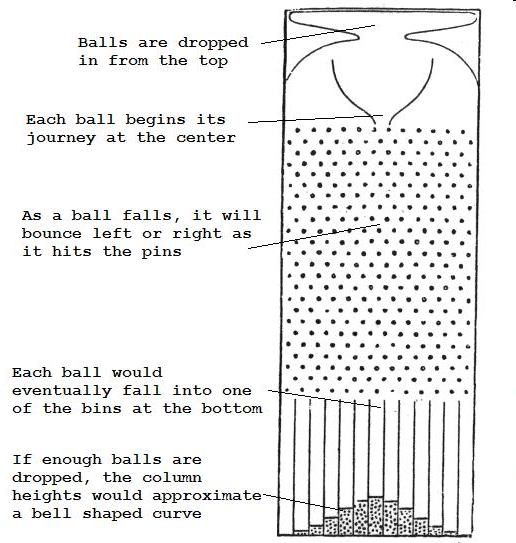
\includegraphics[width=\linewidth,height=4cm,keepaspectratio]{figures/bean_machine.png}

}

\caption{\textbf{Galton's box / quincunx / bean machine}\\
Galton F (1889) \emph{Natural inheritance}. Macmillan, London}

\end{figure}%

\normalsize

\footnotesize \textbf{NB:} \bluenorm{Francis Galton} (1822--1911) was
\bluenorm{Charles Darwin}'s half-cousin (same grandfather: Erasmus
Darwin). He invented correlations, regressions, dog whistles but also
``eugenics''. He coined ``nature vs nurture''. He also discovered
anticyclones and was an explorer (e.g.~Namibia).\normalsize
\end{frame}

\begin{frame}{Measuring uncertainty --- metrics}
\protect\phantomsection\label{measuring-uncertainty-metrics}
\bluebold{Most widely used metrics}
\begin{itemize}
\item{the standard deviation of the estimator = the \blueit{standard error} (SE)}
\end{itemize}

Example, the \blueit{standard error of the mean} (SEM):

\begin{center}
\begin{minipage}[c]{0.3\textwidth}
\begin{callout}
\centering $$\text{SEM} = \dfrac{\text{SD}(\text{sample})}{\sqrt{n}}$$
\end{callout}
\end{minipage}
\end{center}

\textbf{NB:}

\begin{itemize}
\tightlist
\item
  SD quantifies how much measurements vary between each other
\item
  SE quantifies how precise the estimation of a parameter is\\
  (i.e.~how precise the estimation of the mean is if SE is a SEM)
\item
  SEM varies with \(n\) (SD does not)
\end{itemize}
\end{frame}

\begin{frame}{Measuring uncertainty --- metrics}
\protect\phantomsection\label{measuring-uncertainty-metrics-1}
\bluebold{Most widely used metrics}
\begin{itemize}
\item{the standard deviation of the estimator = the \blueit{standard error} (SE)}
\item{the 95\% \blueit{confidence interval} (\ci)\\
$\rightarrow$ by definition, the procedure used for constructing the interval has to deliver a CI that includes the true value of the parameter in 95\% of the time}
\end{itemize}

Example: the \blueit{95\% confidence interval for the mean}

\begin{center}
\begin{minipage}[c]{0.8\textwidth}
\begin{callout}
\bluebold{\ci\ for the mean}\\
= mean ± qt(0.975, df)$\times$SEM\\
(df = degrees of freedom = the number of independent pieces of information available for the estimation = $n-1$ if one mean estimated)\\
$\sim$ mean ± qnorm(0.975)$\times$SEM if $n$ is large or SD(pop) known\\
\bluenorm{$\sim$ mean ± 2$\times$SEM}
\end{callout}
\end{minipage}
\end{center}
\end{frame}

\begin{frame}{Measuring uncertainty --- metrics}
\protect\phantomsection\label{measuring-uncertainty-metrics-2}
\bluebold{Most widely used metrics}
\begin{itemize}
\item{the standard deviation of the estimator = the \blueit{standard error} (SE)}
\item{the 95\% \blueit{confidence interval} (\ci)\\
$\rightarrow$ by definition, the procedure used for constructing the interval has to deliver a CI that includes the true value of the parameter in 95\% of the time}
\end{itemize}

Example: the \blueit{95\% confidence interval for the mean}

\footnotesize

\begin{center}
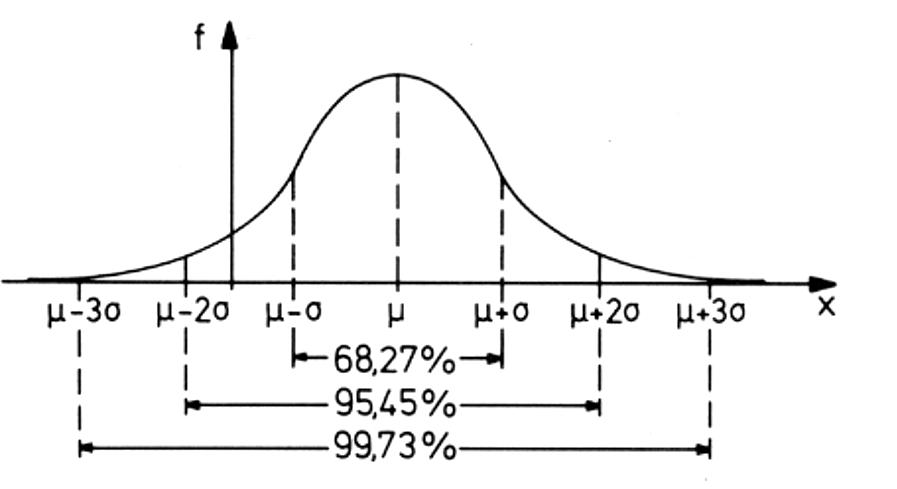
\includegraphics[width=\linewidth,height=3cm,keepaspectratio]{figures/CI.png}
\end{center}

\normalsize
\end{frame}

\section{Likelihood}\label{likelihood}

\begin{frame}{Likelihood --- likelihood vs sampling distribution}
\protect\phantomsection\label{likelihood-likelihood-vs-sampling-distribution}
\bluebold{Likelihood}

the likelihood of a model given the data is equal to the
\blueit{probability density} of those data given assumed parameter
values and distribution of the data:
\(\mathcal{L}(\theta \mid y) = P(y \mid \theta)\)

\vspace{0.5cm}

\begin{callout}
\begin{itemize}
\item the \blueit{sampling distribution} of the estimator shows how much estimates would vary if different samples were collected from the same population
\item the \blueit{likelihood function} instead defines how plausible different estimates are given the sample you have
\end{itemize}
\end{callout}
\end{frame}

\begin{frame}[fragile]{Likelihood --- likelihood computation}
\protect\phantomsection\label{likelihood-likelihood-computation}
\bluebold{Likelihood}

the likelihood of a model given the data is equal to the
\blueit{probability density} of those data given assumed parameter
values and distribution of the data:
\(\mathcal{L}(\theta \mid y) = P(y \mid \theta)\)

\footnotesize

\begin{Shaded}
\begin{Highlighting}[]
\NormalTok{iris }\SpecialCharTok{|\textgreater{}}
  \FunctionTok{filter}\NormalTok{(Species }\SpecialCharTok{==} \StringTok{"versicolor"}\NormalTok{) }\SpecialCharTok{|\textgreater{}} 
  \FunctionTok{mutate}\NormalTok{(}\AttributeTok{density =} \FunctionTok{dnorm}\NormalTok{(}\AttributeTok{x =}\NormalTok{ Petal.Length, }\AttributeTok{mean =} \FloatTok{4.5}\NormalTok{, }\AttributeTok{sd =} \FloatTok{0.5}\NormalTok{),}
         \AttributeTok{log\_density =} \FunctionTok{dnorm}\NormalTok{(}\AttributeTok{x =}\NormalTok{ Petal.Length, }\AttributeTok{mean =} \FloatTok{4.5}\NormalTok{, }\AttributeTok{sd =} \FloatTok{0.5}\NormalTok{, }\AttributeTok{log =} \ConstantTok{TRUE}\NormalTok{)) }\SpecialCharTok{|\textgreater{}} 
  \FunctionTok{summarise}\NormalTok{(}\AttributeTok{Lik =} \FunctionTok{prod}\NormalTok{(density),}
            \AttributeTok{logLik =} \FunctionTok{sum}\NormalTok{(log\_density))}
\end{Highlighting}
\end{Shaded}

\begin{verbatim}
           Lik    logLik
1 1.575195e-17 -38.68957
\end{verbatim}

\normalsize

\textbf{NB:}

\begin{itemize}
\tightlist
\item
  using the log-likelihood produces values that are easier to work with,
  and avoids numerical \blueit{underflow} to zero (which the raw
  likelihood is prone to)
\end{itemize}
\end{frame}

\begin{frame}{Likelihood --- likelihood computation}
\protect\phantomsection\label{likelihood-likelihood-computation-1}
\bluebold{Likelihood}

the likelihood of a model given the data is equal to the
\blueit{probability density} of those data given assumed parameter
values and distribution of the data:
\(\mathcal{L}(\theta \mid y) = P(y \mid \theta)\)

\vspace{0.5cm}

\begin{columns}[T]
\begin{column}{0.33\linewidth}
\footnotesize

\begin{figure}[H]

{\centering \includegraphics[width=\linewidth,height=3.5cm,keepaspectratio]{fundamentals_files/figure-beamer/unnamed-chunk-44-1.pdf}

}

\caption{\footnotesize \(\mu = 4\), \(\sigma = 0.7\)}

\end{figure}%

\normalsize
\end{column}

\pause

\begin{column}{0.33\linewidth}
\footnotesize

\begin{figure}[H]

{\centering \includegraphics[width=\linewidth,height=3.5cm,keepaspectratio]{fundamentals_files/figure-beamer/unnamed-chunk-45-1.pdf}

}

\caption{\footnotesize \(\mu = 4.5\), \(\sigma = 0.7\)}

\end{figure}%

\normalsize
\end{column}

\pause

\begin{column}{0.33\linewidth}
\footnotesize

\begin{figure}[H]

{\centering \includegraphics[width=\linewidth,height=3.5cm,keepaspectratio]{fundamentals_files/figure-beamer/unnamed-chunk-46-1.pdf}

}

\caption{\footnotesize \(\mu = 4.5\), \(\sigma = 0.5\)}

\end{figure}%

\normalsize
\end{column}
\end{columns}
\end{frame}

\begin{frame}[fragile]{Likelihood --- maximum likelihood estimates}
\protect\phantomsection\label{likelihood-maximum-likelihood-estimates}
\bluebold{Maximum likelihood estimates (MLE)}

MLE are estimates that maximise the likelihood function

\begin{columns}[T]
\begin{column}{0.5\linewidth}
\footnotesize

\begin{figure}[H]

{\centering \includegraphics[width=\linewidth,height=3cm,keepaspectratio]{fundamentals_files/figure-beamer/logLikprof-1.pdf}

}

\caption{\footnotesize log-\blueit{likelihood profile} for \(\mu\)}

\end{figure}%

\normalsize
\end{column}

\begin{column}{0.5\linewidth}
\footnotesize

\begin{figure}[H]

{\centering \includegraphics[width=\linewidth,height=3cm,keepaspectratio]{fundamentals_files/figure-beamer/maxlogLik-1.pdf}

}

\caption{\footnotesize joint log-\blueit{likelihood surface} for \(\mu\)
\& \(\sigma\)}

\end{figure}%

\normalsize
\end{column}
\end{columns}

\pause

\begin{itemize}
\tightlist
\item
  in this simple case the MLE of \(\mu\) is the mean and the MLE of
  \(\sigma\) is the SD computed with an n-denominator rather than n−1,
  i.e.~\(\sqrt{\frac{1}{n} \sum_{i=1}^n \left(x_i - \hat{\mu}\right)^2}\),
  or\\
  in R, \texttt{sd(x)*sqrt((n-1)/n)}
\end{itemize}
\end{frame}

\begin{frame}{Likelihood --- maximum likelihood estimates}
\protect\phantomsection\label{likelihood-maximum-likelihood-estimates-1}
\bluebold{Maximum likelihood estimates (MLE)}

MLE are estimates that maximise the likelihood function

\begin{columns}[T]
\begin{column}{0.5\linewidth}
\footnotesize

\begin{figure}[H]

{\centering \includegraphics[width=\linewidth,height=3cm,keepaspectratio]{fundamentals_files/figure-beamer/logLikprof_with_CI-1.pdf}

}

\caption{\footnotesize log-\blueit{likelihood profile} for \(\mu\)}

\end{figure}%

\normalsize
\end{column}

\begin{column}{0.5\linewidth}
\footnotesize

\begin{figure}[H]

{\centering \includegraphics[width=\linewidth,height=3cm,keepaspectratio]{fundamentals_files/figure-beamer/maxlogLik_bis-1.pdf}

}

\caption{\footnotesize joint log-\blueit{likelihood surface} for \(\mu\)
\& \(\sigma\)}

\end{figure}%

\normalsize
\end{column}
\end{columns}

\begin{itemize}
\tightlist
\item
  \ci~can also be derived from this approach
\end{itemize}
\end{frame}

\section{Tests and p-values}\label{tests-and-p-values}

\begin{frame}{Tests and p-values --- principles}
\protect\phantomsection\label{tests-and-p-values-principles}
\vspace{1cm}

\bluebold{Test setup}

\begin{enumerate}
\tightlist
\item
  formulate a null hypothesis H0 for a population:\\
  \(\rightarrow\) H0 is chosen in contrast to the experimental
  hypothesis (H1)
\item
  select and measure a sample
\item
  question: is the sample compatible with H0?

  \begin{itemize}
  \tightlist
  \item
    if ``YES'': by chance or reliably so?
  \item
    if ``NO'': by chance or reliably so?
  \end{itemize}
\end{enumerate}
\end{frame}

\begin{frame}{Tests and p-values --- the null hypothesis}
\protect\phantomsection\label{tests-and-p-values-the-null-hypothesis}
\vspace{1cm}

Ronald Fisher, \emph{The Design of Experiments}, Edinburgh: Oliver and
Boyd, 1935, p.~18

\vspace{0.5cm}

\begin{quote}
"\emph{In relation to any experiment we may speak of this hypothesis as the \bluenorm{null hypothesis}, and it should be noted that the null hypothesis is never proved or established, but is possibly disproved, in the course of experimentation.}

\vspace{1cm}

\emph{Every experiment may be said to exist only in order to give the facts a chance of disproving the null hypothesis.}"
\end{quote}
\end{frame}

\begin{frame}{Tests and p-values --- ``testing by eye'' using \ci}
\protect\phantomsection\label{tests-and-p-values-testing-by-eye-using}
\begin{itemize}
\item
  comparison of one estimated parameter \(\hat{\mu}\) (e.g.~a mean) with
  a fixed value \(\mu_0\)\\
  (\bluenorm{H0: $\hat{\mu} = \mu_0$})

  \begin{itemize}
  \tightlist
  \item
    if \(\mu_0\) is located outside the \ci, then \(\hat{\mu}\) differs
    significantly from \(\mu_0\)\\
    (given \(\alpha\) = 5\%; more on \(\alpha\) later)
  \end{itemize}
\end{itemize}

\pause

\vspace{0.5cm}

\begin{itemize}
\item
  comparison of two estimated parameters \(\hat{\mu}_1\) \&
  \(\hat{\mu}_2\) (e.g.~two means)\\
  (\bluenorm{H0: $\hat{\mu}_1 = \hat{\mu}_2$})

  \begin{enumerate}
  [a.]
  \tightlist
  \item
    if the two \ci~do not overlap, then their means are significantly
    different
  \item
    if the two \ci~overlap, then, mostly, the difference between the
    means is not significant; however, it may happen that, for small
    overlaps, the difference is significant \(\rightarrow\) the \ci~for
    the difference between two means \(\neq\) the difference between two
    individual\ci\\
  \end{enumerate}
\end{itemize}
\end{frame}

\begin{frame}{Tests and p-values --- ``testing by eye'' using \ci}
\protect\phantomsection\label{tests-and-p-values-testing-by-eye-using-1}
\begin{center}
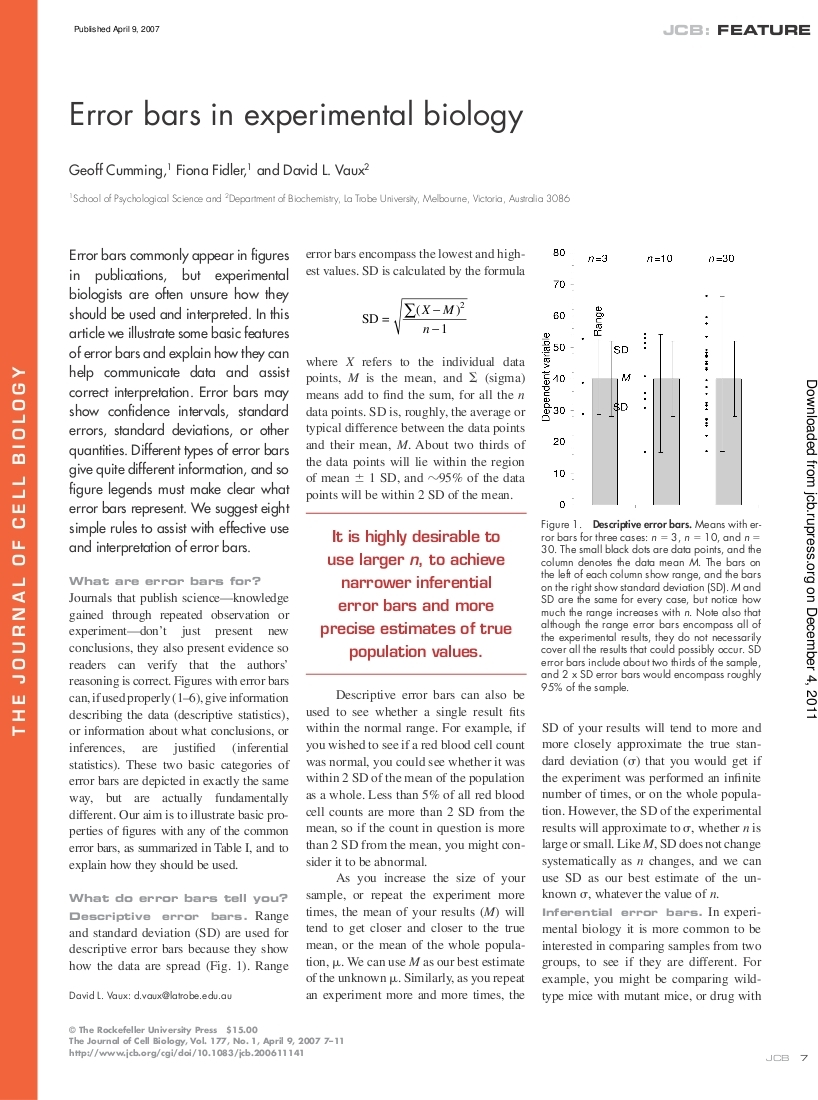
\includegraphics[height=0.8\textheight]{figures/errorbars_paper.jpg}
\end{center}

\footnotesize Cumming et al.~(2007) Error bars in experimental biology.
\emph{Journal of Cell Biology} 177(1): 7--11\normalsize
\end{frame}

\begin{frame}{Principles of statistical tests --- test statistics}
\protect\phantomsection\label{principles-of-statistical-tests-test-statistics}
\begin{enumerate}
\tightlist
\item
  formulate a null hypothesis H0
\item
  define a \bluenorm{test statistic}, a function \(f\) suited to
  quantify the null hypothesis (e.g.~difference of height means)
\item
  select a sample
\item
  hypothesise a distribution of \(f\) under H0; e.g.~\(f\) is assumed to
  be normally distributed (bell-shaped)
\item
  according to H0, mean(\(f\)) = 0; SD(\(f\)) is derived from the
  selected sample
\item
  calculate the value \(v\) = \(f\)(sample) for the sample
\end{enumerate}

\pause

\begin{columns}[T]
\begin{column}{0.55\linewidth}
\begin{callout}
Where is $v$ located in the test distribution?
\begin{itemize}
\item $v$ near the edge: \bluebold{reject} H0
\item $v$ near the middle: \bluebold{do not reject} H0
\end{itemize}

\end{callout}
\end{column}

\begin{column}{0.45\linewidth}
\footnotesize

\begin{center}
\includegraphics[width=\linewidth,height=3cm,keepaspectratio]{fundamentals_files/figure-beamer/unnamed-chunk-47-1.pdf}
\end{center}

\normalsize
\end{column}
\end{columns}
\end{frame}

\begin{frame}{Principles of statistical tests --- \(\alpha\) and
p-value}
\protect\phantomsection\label{principles-of-statistical-tests-alpha-and-p-value}
\footnotesize

\begin{center}
\includegraphics[width=\linewidth,height=2.5cm,keepaspectratio]{fundamentals_files/figure-beamer/unnamed-chunk-48-1.pdf}
\end{center}

\normalsize

\begin{callout}
\bluebold{p-value}

area beyond $v$ (\textcolor{lightgray}{\rule{0.5em}{0.5em}}), i.e. the probability to (randomly) obtain this sample or one with a more extreme departure from H0, if H0 is \bluenorm{true}

\vspace{1em}

\bluebold{significance}

p is regarded \blueit{significant} if p < $\alpha$ (\textcolor{lightgray}{\rule{0.5em}{0.5em}} < \textcolor{red!20!white!100}{\rule{0.5em}{0.5em}}), with \bluenorm{$\alpha$} the \blueit{significance level}, i.e. \bluenorm{the probability of rejecting the null hypothesis when it is true}, previously defined by the researcher (traditionally: $\alpha$ = 0.05)
\end{callout}

\pause

\textcolor{red}{What is the significance outcome of the test illustrated above?}
\end{frame}

\begin{frame}{Principles of statistical tests --- p-value}
\protect\phantomsection\label{principles-of-statistical-tests-p-value}
Data were collected on body height of males \& females and the mean
heights for males and females were calculated.

Result of a t-test: t = 2.7; p = 0.01

\pause

Selection of suggested interpretations:

\begin{enumerate}
\tightlist
\item
  null hypothesis (H0: no difference) absolutely disproved
\item
  p-value reflects the probability of the H0
\item
  experimental hypothesis absolutely proved
\item
  p-value reflects the probability of the experimental hypothesis
  (different means)
\item
  p-value reflects the probability that the decision ``reject H0'' is
  wrong
\item
  for potential replications of the experiment, 99\% of the occasions
  should be significant
\end{enumerate}

\textcolor{red}{Which ones are correct?}
\uncover<3->{\bluenorm{None!} $\rightarrow$ \blueit{frequentist statistics} cannot tell us the probability that a hypothesis is true; we will revisit this in the Bayesian section}
\end{frame}

\begin{frame}{Principles of statistical tests --- significance}
\protect\phantomsection\label{principles-of-statistical-tests-significance}
A difference between H0 and H1 is more easily detectable
(``significant'')

\begin{itemize}
\tightlist
\item
  the larger the size (extent) of the biological effect is
\item
  the smaller the variance of the measurements
\item
  the larger the sample size is
\end{itemize}

\pause

\(\rightarrow\) \bluenorm{small differences} can be
\bluenorm{significant} with a small variance and/or a large sample
size\\
\(\rightarrow\) \bluenorm{large differences} can be
\bluenorm{insignificant} with a large variance and/or a small sample
size

\pause

\vspace{0.5cm}

To evaluate a difference between H0 and H1 one has to consider:

\begin{itemize}
\tightlist
\item
  the \blueit{effect size}
\item
  the p-value together with sample size \& variance\\
  (which together shape the \blueit{variance of the test statistics})
\end{itemize}
\end{frame}

\begin{frame}{Principles of statistical tests --- p-value}
\protect\phantomsection\label{principles-of-statistical-tests-p-value-1}
Data were collected on body height of males \& females, the mean heights
for males (M) and females (F) were calculated. All four results listed
are possible:

\begin{center}
\begin{tabular}{lll}
M = 180 & F = 175 & p = 0.001 \\
\textcolor{red}{M = 180} & \textcolor{red}{F = 175} & \textcolor{red}{p = 0.100} \\
\textcolor{red}{M = 180.0} & \textcolor{red}{F = 179.9} & \textcolor{red}{p = 0.001} \\
\textcolor{red}{M = 175} & \textcolor{red}{F = 180} & \textcolor{red}{p = 0.049} \\
\end{tabular}
\end{center}

\textcolor{red}{Why?}

\pause

\bluebold{Potential reasons for unexpected results}

\begin{itemize}
\tightlist
\item
  chance (sample not representative of the population)
\item
  sample is systematically biased (volleyball team)
\item
  sample too small or even very large
\item
  improper test
\item
  test requirements not met
\end{itemize}
\end{frame}

\begin{frame}{Principles of statistical tests --- p-value}
\protect\phantomsection\label{principles-of-statistical-tests-p-value-2}
Data were collected on body height of males \& females, the mean heights
for males (M) and females (F) were calculated. All four results listed
are possible:

\begin{center}
\begin{tabular}{lll}
M = 180 & F = 175 & p = 0.001 \\
\textcolor{red}{M = 180} & \textcolor{red}{F = 175} & \textcolor{red}{p = 0.100} \\
\textcolor{red}{M = 180.0} & \textcolor{red}{F = 179.9} & \textcolor{red}{p = 0.001} \\
\textcolor{red}{M = 175} & \textcolor{red}{F = 180} & \textcolor{red}{p = 0.049} \\
\end{tabular}
\end{center}

\textcolor{red}{Why?}

\(\rightarrow\) The evaluation of a test result requires:

\begin{itemize}
\tightlist
\item
  p-value
\item
  effect size (relevant effect?)
\item
  sample (proper selection method chosen?)
\item
  sample size
\item
  test and whether its requirements were met
\end{itemize}
\end{frame}

\begin{frame}{Principles of statistical tests --- summary on p-values}
\protect\phantomsection\label{principles-of-statistical-tests-summary-on-p-values}
\textbf{ASA statement on statistical significance and p-values (Wasserstein 2016)}
\footnotesize \url{https://amstat.tandfonline.com/doi/pdf/10.1080/00031305.2016.1154108}\normalsize

\begin{itemize}
\tightlist
\item
  p-values can indicate how incompatible the data are with a specified
  statistical model
\item
  p-values do not measure the probability that the studied hypothesis is
  true, or the probability that the data were produced by random chance
  alone
\item
  scientific conclusions and business or policy decisions should not be
  based only on whether a p-value passes a specific threshold
\item
  proper inference requires full reporting and transparency
\item
  a p-value, or statistical significance, does not measure the size of
  an effect or the importance of a result
\item
  by itself, a p-value does not provide a good measure of evidence
  regarding a model or hypothesis
\end{itemize}
\end{frame}

\begin{frame}{Principles of statistical tests --- one-sided vs two-sided
tests}
\protect\phantomsection\label{principles-of-statistical-tests-one-sided-vs-two-sided-tests}
\bluebold{Two-sided hypothesis} (e.g.~body height): H0: males = females;
H1: males \(\neq\) females

\begin{itemize}
\tightlist
\item
  H0 is rejected only if the test statistic deviates in
  \bluebold{either direction}
\item
  ``extreme'' means that the test statistic in the 5\%-region (i.e.~the
  \blueit{rejection region})\\
  \(\rightarrow\) the ``rejection region'' is split into 2 \(\times\)
  2.5\%-regions
\end{itemize}

\vspace{0.5cm}

\footnotesize

\begin{figure}[H]

{\centering \includegraphics[width=\linewidth,height=2.5cm,keepaspectratio]{fundamentals_files/figure-beamer/unnamed-chunk-49-1.pdf}

}

\caption{two-sided rejection regions (if the test statistic follows a
standard normal distribution)}

\end{figure}%

\normalsize
\end{frame}

\begin{frame}{Principles of statistical tests --- one-sided vs two-sided
tests}
\protect\phantomsection\label{principles-of-statistical-tests-one-sided-vs-two-sided-tests-1}
\bluebold{One-sided hypothesis} (e.g.~body height): H0: males = females;
H1: males \textgreater{} females

\begin{itemize}
\tightlist
\item
  H0 is rejected only if the test statistic deviates in
  \bluebold{one direction}
\item
  ``extreme'' means that the test statistic in the 5\%-region (i.e.~the
  \blueit{rejection region})\\
  \(\rightarrow\) the ``rejection region'' is at one side of the test
  distribution
\end{itemize}

\vspace{0.5cm}

\footnotesize

\begin{figure}[H]

{\centering \includegraphics[width=\linewidth,height=2.5cm,keepaspectratio]{fundamentals_files/figure-beamer/unnamed-chunk-50-1.pdf}

}

\caption{one-sided rejection region (if the test statistic follows a
standard normal distribution)}

\end{figure}%

\normalsize

\pause

\vspace{-0.5cm}

\begin{callout}
One-sided hypotheses are \bluenorm{easier to reject} $\rightarrow$ use one-sided tests only if the opposite case can be very confidently excluded!
\end{callout}
\end{frame}

\begin{frame}{Principles of statistical tests --- interpretation}
\protect\phantomsection\label{principles-of-statistical-tests-interpretation}
\bluebold{How to interpret the result of null hypothesis significance testing (NHST)?}\\
(e.g.~the outcome of a t-test between the height of males and females)

\begin{itemize}
\tightlist
\item
  your test is significant \(p\leq0.05\)\\
  \(\rightarrow\) it supports that the (population) means of the two
  groups differ
\end{itemize}

\pause

\begin{itemize}
\tightlist
\item
  your test is not significant (\(p>0.05\))\\
  \(\rightarrow\) it supports that the (population) means are the same
  across the two groups
\end{itemize}

\pause

\bluebold{What is wrong with this classical interpretation of a lack of significance?}

\begin{itemize}
\tightlist
\item
  the \bluenorm{null} hypothesis is \bluenorm{dull}\\
  \(\rightarrow\) two groups most likely differ in reality, even if you
  don't have the power to detect the difference!
\end{itemize}
\end{frame}

\begin{frame}{Principles of statistical tests --- interpretation}
\protect\phantomsection\label{principles-of-statistical-tests-interpretation-1}
\bluebold{How to interpret the result of null hypothesis significance testing (NHST)?}\\
(e.g.~the outcome of a t-test between the height of males and females)

\begin{itemize}
\item
  your test is significant \(p\leq0.05\)\\
  \(\rightarrow\) it supports that the (population) means of the two
  groups differ
\item
  your test is not significant (\(p>0.05\))\\
  \(\rightarrow\) it supports that the (population) means are the same
  across the two groups
\end{itemize}

\bluebold{What is wrong with this classical interpretation of a lack of significance?}

\begin{callout}
\bluebold{Refined interpretation}\\
$p>0.05$ doesn't mean there is no effect\\
$\rightarrow$ your data are equally compatible with the effect going the other way\\
$\rightarrow$\bluenorm{you cannot yet tell the direction of the true effect!}
\end{callout}
\end{frame}

\section{Multiple testing}\label{multiple-testing}

\begin{frame}{Multiple testing --- is alpha everything?}
\protect\phantomsection\label{multiple-testing-is-alpha-everything}
\textcolor{red}{\textbf{Question 1} if the null hypothesis is true in the population, what will be the probability to detect on a sample a significant departure from the null hypothesis (with $\alpha$ = 0.05)?}

\centering \bluebold{P(reject H0 | H0) = ?}

\raggedright
\vspace{0.5cm}

\pause

\textcolor{red}{\textbf{Question 2} if the null hypothesis is true in the population, what will be the probability to detect among 10 samples at least one showing a significant departure from the null hypothesis (with $\alpha$ = 0.05)?}

\vspace{1cm}

Cue: think about the biologist trying to catch a bird\ldots{}
\end{frame}

\begin{frame}[fragile]{Multiple testing --- is alpha everything?}
\protect\phantomsection\label{multiple-testing-is-alpha-everything-1}
\textcolor{red}{\textbf{Question 2} if the null hypothesis is true in the population, what will be the probability to detect among 10 samples at least one showing a significant departure from the null hypothesis (with $\alpha$ = 0.05)?}

\begin{columns}[T]
\begin{column}{0.6\linewidth}
\footnotesize

\begin{Shaded}
\begin{Highlighting}[]
\DecValTok{1} \SpecialCharTok{{-}} \FunctionTok{dbinom}\NormalTok{(}\AttributeTok{x =} \DecValTok{0}\NormalTok{, }\AttributeTok{size =} \DecValTok{10}\NormalTok{, }\AttributeTok{prob =} \FloatTok{0.05}\NormalTok{)}
\end{Highlighting}
\end{Shaded}

\begin{verbatim}
[1] 0.4012631
\end{verbatim}

\normalsize
\end{column}

\begin{column}{0.4\linewidth}
\footnotesize

\begin{figure}[H]

{\centering \includegraphics[width=\linewidth,height=4cm,keepaspectratio]{fundamentals_files/figure-beamer/unnamed-chunk-52-1.pdf}

}

\caption{\footnotesize (H0 is assumed true)}

\end{figure}%

\normalsize
\end{column}
\end{columns}

\pause

How many experiments testing the same question are being conducted?
\end{frame}

\begin{frame}{Multiple testing --- is alpha everything?}
\protect\phantomsection\label{multiple-testing-is-alpha-everything-2}
\footnotesize

\begin{figure}[H]

{\centering 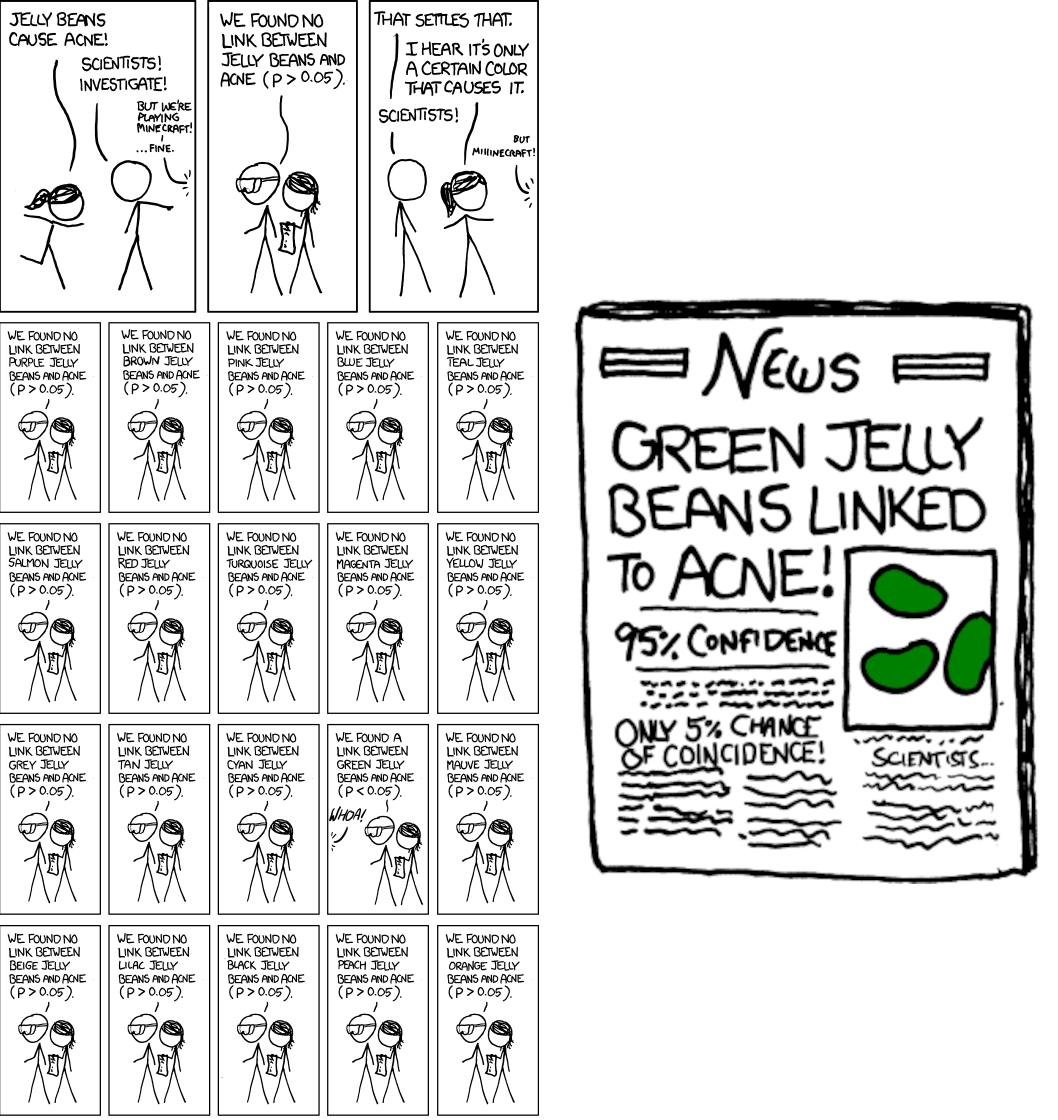
\includegraphics[width=\linewidth,height=7cm,keepaspectratio]{figures/xkcd_significance_wide.png}

}

\caption{\footnotesize \copyright~\url{xkcd.com/882}}

\end{figure}%

\normalsize
\end{frame}

\begin{frame}{Multiple testing --- what to do?}
\protect\phantomsection\label{multiple-testing-what-to-do}
\begin{itemize}
\tightlist
\item
  avoid if possible!
\item
  restrict the number of tests during the planning of analyses to
  ``important'' tests
\item
  do not ``generate'' significant differences afterwards by excluding
  the non-significant tests\\
  \(\rightarrow\) it is a recipe for generating false positives and thus
  a recipe for disasters (unethical \& potentially harmful)
\item
  there are special adjustment procedures if you must perform multiple
  testing
\end{itemize}
\end{frame}

\begin{frame}[fragile]{Multiple testing --- the Bonferroni correction}
\protect\phantomsection\label{multiple-testing-the-bonferroni-correction}
\begin{callout}
\bluebold{Bonferroni correction}\\
for $m$ comparisons, test the single p-value not for $\alpha=0.05$, but for $\alpha=0.05/m$
\end{callout}

Example: in the case of 10 tests, \(\alpha=0.05/10 = 0.005\)

\footnotesize

\begin{center}
\includegraphics[width=\linewidth,height=3cm,keepaspectratio]{fundamentals_files/figure-beamer/unnamed-chunk-54-1.pdf}
\end{center}

\normalsize

\pause

\begin{itemize}
\tightlist
\item
  the Bonferroni correction makes it much harder to detect real
  effects\\
  (we will define this cost, a decrease in \blueit{statistical power},
  precisely soon)
\item
  alternatives exist and differ in their trade-off between type 1 \& 2
  errors (see \texttt{?p.adjust})
\end{itemize}
\end{frame}

\begin{frame}[fragile]{Multiple testing --- replication vs multiple
testing}
\protect\phantomsection\label{multiple-testing-replication-vs-multiple-testing}
Why should you replicate positive experiments
(i.e.~\blueit{cross validation}) but not negative ones
(i.e.~\blueit{multiple testing})?

\begin{itemize}
\tightlist
\item
  if \(\alpha\) is 0.05, what is the probability of obtaining at least
  one false positive after 3 experiments?
\end{itemize}

\footnotesize

\begin{Shaded}
\begin{Highlighting}[]
\DecValTok{1} \SpecialCharTok{{-}} \FunctionTok{dbinom}\NormalTok{(}\AttributeTok{x =} \DecValTok{0}\NormalTok{, }\AttributeTok{size =} \DecValTok{3}\NormalTok{, }\AttributeTok{prob =} \FloatTok{0.05}\NormalTok{) }\CommentTok{\# = 1 {-} 0.95\^{}3}
\end{Highlighting}
\end{Shaded}

\begin{verbatim}
[1] 0.142625
\end{verbatim}

\normalsize

\pause

\begin{itemize}
\tightlist
\item
  if \(\alpha\) is 0.05, what is the probability of only obtaining false
  positives after 3 experiments?
\end{itemize}

\footnotesize

\begin{Shaded}
\begin{Highlighting}[]
\FunctionTok{dbinom}\NormalTok{(}\AttributeTok{x =} \DecValTok{3}\NormalTok{, }\AttributeTok{size =} \DecValTok{3}\NormalTok{, }\AttributeTok{prob =} \FloatTok{0.05}\NormalTok{) }\CommentTok{\# = 0.05\^{}3}
\end{Highlighting}
\end{Shaded}

\begin{verbatim}
[1] 0.000125
\end{verbatim}

\normalsize

\pause

\begin{callout}
cross validation reduces the risk of false positive while multiple testing increases it!
\end{callout}
\end{frame}

\section{Statistical power}\label{statistical-power}

\begin{frame}{Statistical power --- type 1 and type 2 errors}
\protect\phantomsection\label{statistical-power-type-1-and-type-2-errors}
\begin{center}
\begin{minipage}[c]{0.7\linewidth}
\begin{callout}
\begin{tabular}{p{2cm}p{3cm}p{3cm}}
prob. to & \makecell[c]{accept H0} & \makecell[c]{reject H0}\\
given that & & \\
H0 true & \cellcolor{okgreen}\makecell[c]{true negative}& \cellcolor{bad}\makecell[c]{false positive}\\
H0 false & \cellcolor{bad}\makecell[c]{false negative} & \cellcolor{okgreen}\makecell[c]{true positive}\\
\end{tabular}
\end{callout}
\end{minipage}
\end{center}

\pause

\vspace{0.5cm}

Many metrics can be deduced from this table:

{\def\LTcaptype{none} % do not increment counter
\begin{longtable}[]{@{}ll@{}}
\toprule\noalign{}
Metric & Definition \\
\midrule\noalign{}
\endhead
\blueit{accuracy} & true / all \\
\blueit{sensitivity} & true positive / H0 false \\
\blueit{specificity} & true negative / H0 true \\
\blueit{precision} & true positive / reject H0 \\
\blueit{false discovery rate} & false positive / reject H0 \\
\bottomrule\noalign{}
\end{longtable}
}
\end{frame}

\begin{frame}{Statistical power --- type 1 and type 2 errors}
\protect\phantomsection\label{statistical-power-type-1-and-type-2-errors-1}
\begin{center}
\begin{minipage}[c]{0.7\linewidth}
\begin{callout}
\begin{tabular}{p{2cm}p{3cm}p{3cm}}
prob. to & \makecell[c]{accept H0} & \makecell[c]{reject H0}\\
given that & & \\
H0 true & \cellcolor{okgreen}\makecell[c]{true negative}& \cellcolor{bad}\makecell[c]{false positive}\\
H0 false & \cellcolor{bad}\makecell[c]{false negative} & \cellcolor{okgreen}\makecell[c]{true positive}\\
\end{tabular}
\end{callout}
\end{minipage}
\end{center}

\vspace{0.5cm}

\begin{center}
\begin{tabular}{p{2cm}p{3cm}p{3cm}}
prob. to & \makecell[c]{accept H0} & \makecell[c]{reject H0}\\
given that & & \\
H0 true & \cellcolor{okgreen}\makecell[c]{1 -- $\alpha$} & \cellcolor{bad}\makecell[c]{$\alpha$ = \blueit{type 1 error}}\ \\
H0 false & \cellcolor{bad}\makecell[c]{$\beta$ = \blueit{type 2 error}} & \cellcolor{okgreen}\makecell[c]{1 -- $\beta$ = \blueit{power}} \\
\end{tabular}
\end{center}

\pause

\textbf{NB:}

\begin{itemize}
\tightlist
\item
  if avoiding false negatives matters most, one should increase the
  power
\item
  if avoiding false positives matters most, one should decrease
  \(\alpha\)
\end{itemize}

\ldots{} but there is a \bluenorm{trade-off} between the two, see next!
\end{frame}

\begin{frame}{Statistical power --- trade-off between false positives \&
negatives}
\protect\phantomsection\label{statistical-power-trade-off-between-false-positives-negatives}
\footnotesize

\normalsize

\begin{itemize}
\tightlist
\item
  we can compute the distribution of the test statistic under H0
\item
  let's also imagine that we know it under H1 (although it is not
  possible in practice)
\end{itemize}

\vspace{0.5cm}

\footnotesize

\begin{figure}[H]

{\centering \includegraphics[width=\linewidth,height=4cm,keepaspectratio]{fundamentals_files/figure-beamer/unnamed-chunk-57-1.pdf}

}

\caption{baseline situation}

\end{figure}%

\normalsize
\end{frame}

\begin{frame}{Statistical power --- trade-off between false positives \&
negatives}
\protect\phantomsection\label{statistical-power-trade-off-between-false-positives-negatives-1}
\begin{itemize}
\tightlist
\item
  we can compute the distribution of the test statistic under H0
\item
  let's also imagine that we know it under H1 (although it is not
  possible in practice)
\end{itemize}

\vspace{0.5cm}

\footnotesize

\begin{figure}[H]

{\centering \includegraphics[width=\linewidth,height=4cm,keepaspectratio]{fundamentals_files/figure-beamer/unnamed-chunk-58-1.pdf}

}

\caption{\(\alpha\) increases \(\rightarrow\) power increases but false
positives increase too}

\end{figure}%

\normalsize
\end{frame}

\begin{frame}{Statistical power --- trade-off between false positives \&
negatives}
\protect\phantomsection\label{statistical-power-trade-off-between-false-positives-negatives-2}
\begin{itemize}
\tightlist
\item
  we can compute the distribution of the test statistic under H0
\item
  let's also imagine that we know it under H1 (although it is not
  possible in practice)
\end{itemize}

\vspace{0.5cm}

\footnotesize

\begin{figure}[H]

{\centering \includegraphics[width=\linewidth,height=4cm,keepaspectratio]{fundamentals_files/figure-beamer/unnamed-chunk-59-1.pdf}

}

\caption{\(\alpha\) decreases \(\rightarrow\) false positives decrease
but the power decreases too}

\end{figure}%

\normalsize
\end{frame}

\begin{frame}{Statistical power --- trade-off between false positives \&
negatives}
\protect\phantomsection\label{statistical-power-trade-off-between-false-positives-negatives-3}
\begin{itemize}
\tightlist
\item
  we can compute the distribution of the test statistic under H0
\item
  let's also imagine that we know it under H1 (although it is not
  possible in practice)
\end{itemize}

\vspace{0.5cm}

\footnotesize

\begin{figure}[H]

{\centering \includegraphics[width=\linewidth,height=4cm,keepaspectratio]{fundamentals_files/figure-beamer/unnamed-chunk-60-1.pdf}

}

\caption{the trade-off decreases when the effect size is stronger}

\end{figure}%

\normalsize
\end{frame}

\begin{frame}{Statistical power --- trade-off between false positives \&
negatives}
\protect\phantomsection\label{statistical-power-trade-off-between-false-positives-negatives-4}
\begin{itemize}
\tightlist
\item
  we can compute the distribution of the test statistic under H0
\item
  let's also imagine that we know it under H1 (although it is not
  possible in practice)
\end{itemize}

\vspace{0.5cm}

\footnotesize

\begin{figure}[H]

{\centering \includegraphics[width=\linewidth,height=4cm,keepaspectratio]{fundamentals_files/figure-beamer/unnamed-chunk-61-1.pdf}

}

\caption{the trade-off decreases when the variances are smaller}

\end{figure}%

\normalsize
\end{frame}

\begin{frame}{Statistical power --- planning of sample size}
\protect\phantomsection\label{statistical-power-planning-of-sample-size}
\bluebold{Ideal sample size?}

\begin{itemize}
\tightlist
\item
  the power of any statistical test depends on sample size
\item
  the sample should be large enough to detect a reasonable effect with
  an acceptably high probability
\end{itemize}

\vspace{1cm}

\bluebold{Why planning?}

\begin{itemize}
\tightlist
\item
  sample size planning \bluenorm{before} data collection serves to
  prevent falsely insignificant results as a consequence of a sample
  being too small, and to prevent wasting time, effort and lives because
  a larger than necessary sample is being studied
\end{itemize}
\end{frame}

\begin{frame}{Statistical power --- planning of sample size}
\protect\phantomsection\label{statistical-power-planning-of-sample-size-1}
\bluebold{Interacting characteristics affecting a test result}

\begin{enumerate}
\tightlist
\item
  power: common default: 0.8
\item
  \(\alpha\)-risk: commonly 0.05
\item
  \bluenorm{effect size}: minimum relevant value
\item
  \bluenorm{standard deviation}: preliminary analysis
\item
  \bluebold{sample size}: to be estimated
\end{enumerate}

\vspace{0.5cm}

\pause

\bluebold{Frequent problems}

\begin{itemize}
\tightlist
\item
  what is the minimum relevant effect?
\item
  how to estimate the standard deviation (SD) without a preliminary
  analysis?
\end{itemize}
\end{frame}

\begin{frame}[fragile]{Statistical power --- power analysis}
\protect\phantomsection\label{statistical-power-power-analysis}
\bluebold{Preparation}

\begin{itemize}
\tightlist
\item
  get information about the (potential) SD of the sample
\item
  define the size of the minimum relevant effect
\end{itemize}

\vspace{0.5cm}

\bluebold{Possible methods to plan the sample size}

\begin{itemize}
\tightlist
\item
  use equations quantifying the relationship between \(\alpha\)-risk,
  \(\beta\)-risk, effect size and SD for the test to be applied
  (e.g.~\texttt{power.t.test()} for a t-test)
\item
  simulate measurements and apply your test (works for all tests!)
\end{itemize}
\end{frame}

\begin{frame}{Statistical power --- power analysis by simulation}
\protect\phantomsection\label{statistical-power-power-analysis-by-simulation}
\(\rightarrow\) for known \(\alpha\) and \(n\), the power can be
determined by simulation, even if the distribution of the test statistic
is unknown

\vspace{0.5cm}

\bluebold{Procedure}

\begin{enumerate}
\tightlist
\item
  calculate the test statistic presuming H1 for many randomly generated
  samples of size \(n\)
\item
  determine the percentage of test results under H1, which are
  significant
\end{enumerate}

\pause

\vspace{0.5cm}

\bluebold{Constraint}

you must have some idea concerning the process generating the data in
order to generate the samples by an algorithm
\end{frame}

\begin{frame}{Summary}
\protect\phantomsection\label{summary}
What should you know before performing a statistical test?

\begin{callout}
\begin{itemize}
\item \bluenorm{which question should be answered?}\\
more precisely: what is my \bluenorm{null hypothesis}?
\item for which \bluenorm{population} is the question to be answered?
\item which minimum \bluenorm{effect size} can be regarded as \bluenorm{relevant}?
\item which is the \bluenorm{right test} to find the answer?
\item which \bluenorm{assumptions} does the test statistic make about the population?
\item which \bluenorm{requirements} apply to my \bluenorm{sample} in order
\begin{enumerate}
\item to conform with the assumptions for the test statistic?
\item to represent the population adequately?
\end{enumerate}
\end{itemize}
\end{callout}
\end{frame}

\section{Interlude}\label{interlude}

\begin{frame}{Interlude --- is power everything?}
\protect\phantomsection\label{interlude-is-power-everything}
Imagine an \bluenorm{ideal situation}: we perform a clinical test to
diagnose a specific cancer with a known \bluenorm{power of 99\%} and we
set a significance threshold \bluenorm{$\alpha$ at 0.05}

\textcolor{red}{\textbf{Question 1} what is the probability of being positive at the test when having the cancer?}

\centering \bluebold{P(reject H0 | H1) = ?}

\raggedright
\vspace{0.5cm}

\pause

\textcolor{red}{\textbf{Question 2} what is the probability that a person with a positive test has the cancer?}

\centering
\bluebold{P(H1 | reject H0) = ?}

\raggedright

\vspace{0.5cm}

\textbf{NB:} P(H1 \textbar{} reject H0) \(\neq\) P(reject H0 \textbar{}
H1)
\end{frame}

\begin{frame}{Interlude --- is power everything?}
\protect\phantomsection\label{interlude-is-power-everything-1}
\textcolor{red}{\textbf{Question 2} what is the probability that a person with a positive test has the cancer?}

\begin{center}
\resizebox{0.5\linewidth}{!}{%
\begin{forest}
for tree={
  align=center,
  parent anchor=south,
  child anchor=north,
  edge={-latex, thick},
  l sep=10mm,
  s sep=2mm,
  font=\small,
}
[{population}
  [{cancer}, edge label={node[midway, anchor=east, xshift=-10pt, font=\small]{$P(\mathrm{cancer})$}}
    [{test $\oplus$\\(true positive)}, draw, rounded corners, fill=gray!10,
      edge label={node[midway, anchor=east, xshift=-10pt, font=\scriptsize, align=center]{$1 - \beta$}}]
    [{test $\circleddash$\\ (false negative)}, draw, rounded corners, fill=gray!10,
      edge label={node[midway, anchor=west, xshift=10pt,  font=\scriptsize, align=center]{$\beta$}}]
  ]
  [{no cancer}, edge label={node[midway, anchor=west, xshift=10pt, font=\small]{$P(\mathrm{no\ cancer})$}}
    [{test $\oplus$\\(false positive)}, draw, rounded corners, fill=gray!10,
      edge label={node[midway, anchor=east, xshift=-10pt, font=\scriptsize, align=center]{$\alpha$}}]
    [{test $\circleddash$\\ (true negative)}, draw, rounded corners, fill=gray!10,
      edge label={node[midway, anchor=west, xshift=10pt, font=\scriptsize, align=center]{$1 - \alpha$}}]
  ]
]
\end{forest}
}
\end{center}

\pause

\vspace{0.5cm}

\(P(\mathrm{cancer}|\oplus) = \frac{\mathrm{true\ positive}}{\mathrm{true\ positive} + \mathrm{false\ positive}} =  \frac{(1 - \beta) \times P(\mathrm{cancer})}{(1 - \beta) \times P(\mathrm{cancer}) + \alpha \times P(\mathrm{no\ cancer})}\)

\begin{itemize}
\tightlist
\item
  to chain probabilities (i.e.~``and'') you need to multiply them
\item
  to combine probabilities (i.e.~``or'') you need to add them
\item
  the vertical bar ``\textbar{}'' means ``conditional to''
  (i.e.~\(P(y|x)\) is the probability to observe \(y\) when \(x\) has
  occurred)
\end{itemize}
\end{frame}

\begin{frame}{Interlude --- is power everything?}
\protect\phantomsection\label{interlude-is-power-everything-2}
\textcolor{red}{\textbf{Question 2} what is the probability that a person with a positive test has the cancer?}

\footnotesize

\begin{figure}[H]

{\centering \includegraphics[width=\linewidth,height=4cm,keepaspectratio]{fundamentals_files/figure-beamer/unnamed-chunk-62-1.pdf}

}

\caption{\footnotesize (computation assuming a power of 99\% and
\(\alpha\) of 5\%)}

\end{figure}%

\normalsize

\(\rightarrow\) it depends on the
\bluenorm{frequency of cancer in the population}!

\pause

\textbf{NB:} you of all people should not be too surprised\dots~think of
\bluenorm{camera traps}!!
\end{frame}

\begin{frame}{Interlude --- a parallel with occupancy models}
\protect\phantomsection\label{interlude-a-parallel-with-occupancy-models}
\textcolor{red}{\textbf{Question 3} what is the probability that a species not observed is not there?}

\begin{center}
\resizebox{0.5\linewidth}{!}{%
\begin{forest}
for tree={
  align=center,
  parent anchor=south,
  child anchor=north,
  edge={-latex, thick},
  l sep=10mm,
  s sep=2mm,
  font=\small,
}
[{population}
  [{presence}, edge label={node[midway, anchor=east, xshift=-10pt, font=\small]{$P(\mathrm{occupancy}) = \psi$}}
    [{detected\\(true positive)}, draw, rounded corners, fill=gray!10,
      edge label={node[midway, anchor=east, yshift=-5pt, xshift=-10pt, font=\scriptsize, align=center]{$P(\mathrm{detection}) = p_{11}$}}]
    [{not detected\\ (false negative)}, draw, rounded corners, fill=gray!10,
      edge label={node[midway, anchor=west, yshift=-5pt, xshift=10pt,  font=\scriptsize, align=center]{$1 - p_{11}$}}]
  ]
  [{absence}, edge label={node[midway, anchor=west, xshift=10pt, font=\small]{$1 - \psi$}}
    [{"detected"\\(false positive)}, draw, rounded corners, fill=gray!10,
      edge label={node[midway, anchor=east, yshift=10pt, xshift=10pt, font=\scriptsize]{$P(\mathrm{spurious\ detection}) = p_{10}$}}]
    [{not detected\\ (true negative)}, draw, rounded corners, fill=gray!10,
      edge label={node[midway, anchor=west, yshift=10pt, xshift=-10pt, font=\scriptsize]{$1 - p_{10}$}}]
  ]
]
\end{forest}
}
\end{center}

\pause

\vspace{0.5cm}

\(P(\mathrm{absence}|\mathrm{not\ detected}) = \frac{\mathrm{true\ negative}}{\mathrm{true\ negative} + \mathrm{false\ negative}}\)

\(P(\mathrm{absence}|\mathrm{not\ detected}) = \frac{(1 - p_{10}) \times (1 - \psi)}{(1 - p_{10})\times (1 - \psi) + (1 - p_{11})\times \psi}\)

\(P(\mathrm{absence}|\mathrm{not\ detected}) \sim \frac{1 \times (1 - \psi)}{1 \times (1 - \psi) + (1 - p_{11})\times \psi} = \frac{1-\psi}{1-p_{11}\psi}\)
if \(p_{10} \sim 0\)
\end{frame}

\begin{frame}{Interlude --- a parallel with occupancy models}
\protect\phantomsection\label{interlude-a-parallel-with-occupancy-models-1}
\textcolor{red}{\textbf{Question 3} what is the probability that a species not observed is not there?}

\footnotesize

\begin{figure}[H]

{\centering \includegraphics[width=\linewidth,height=4cm,keepaspectratio]{fundamentals_files/figure-beamer/unnamed-chunk-63-1.pdf}

}

\caption{\footnotesize (computation assuming no spurious detection)}

\end{figure}%

\normalsize

\(\rightarrow\) the probability of \bluenorm{absence} at a site where
the species is not detected strongly depends on the
\bluenorm{probability of observation} at sites where the species is
\bluenorm{present}!
\end{frame}

\section{Bayesian statistics}\label{bayesian-statistics}

\begin{frame}{Bayesian statistics --- what are Bayesian statistics?}
\protect\phantomsection\label{bayesian-statistics-what-are-bayesian-statistics}
Bayesian statistics are an alternative branch of statistics where data
analyses and parameter estimation are based on \blueit{Bayes' theorem}

\pause

\begin{itemize}
\tightlist
\item
  large differences exist between alternative approaches:
\end{itemize}

\begin{center}
\begin{small}
\begin{tabular}{|lcc|}
\hline & \blueit{frequentist statistics} & \blueit{Bayesian statistics}\\
\bluenorm{probability interpretation} & relative frequency of an outcome & degrees of belief \\
\bluenorm{hypothesis status} & either true or false & more or less probable\\
\bluenorm{data representation} & random draw from population & fixed\\
\bluenorm{parameter representation} & fixed value in population & probability distribution\\
\bluenorm{external information} & not formally incorporated & prior distributions\\
\bluenorm{uncertainty measurement} & confidence intervals & credible intervals\\
\hline
\end{tabular}
\end{small}
\end{center}

\pause

\begin{itemize}
\tightlist
\item
  \bluenorm{epistemological differences} are interesting/intriguing but
  they are not the reason why Bayesian statistics have become
  increasingly popular in Ecology \& Conservation\\
  \(\rightarrow\) you will discover the \bluenorm{practical reason} soon
  enough
\end{itemize}
\end{frame}

\begin{frame}{Bayesian statistics --- Bayes' theorem}
\protect\phantomsection\label{bayesian-statistics-bayes-theorem}
Abstract version of \blueit{Bayes' theorem}

\begin{columns}[T]
\begin{column}{0.5\linewidth}
\begin{center}
\resizebox{!}{0.4\textheight}{%
\begin{forest}
for tree={
  align=center,
  parent anchor=south,
  child anchor=north,
  edge={-latex, thick},
  l sep=10mm,
  s sep=10mm,
  font=\small,
}
[{population}
  [{$\mathrm{A}$}, edge label={node[midway, anchor=east, xshift=-5pt, font=\small]{{$P(\mathrm{A})$}}}
    [{$\mathrm{B}$}, edge label={node[midway, anchor=east, yshift=-5pt, xshift=-5pt, font=\scriptsize, align=center]{$P(\mathrm{B}|\mathrm{A})$}}]
    [{$\neg \mathrm{B}$}, edge label={node[midway, anchor=west, yshift=-5pt, xshift=5pt, font=\scriptsize, align=center]{$1-P(\mathrm{B}|\mathrm{A})$}}]
  ]
  [{$\neg \mathrm{A}$}, edge label={node[midway, anchor=west, xshift=5pt, font=\small]{$1 - P(\mathrm{A})$}}
    [{$\mathrm{B}$}, edge label={node[midway, anchor=east, yshift=10pt, xshift=5pt, font=\scriptsize]{$P(\mathrm{B}|\neg\mathrm{A})$}}]
    [{$\neg \mathrm{B}$}, edge label={node[midway, anchor=west, yshift=10pt, xshift=-5pt, font=\scriptsize]{$1 - P(\mathrm{B}|\neg\mathrm{A})$}}]
  ]
]
\end{forest}
}
\end{center}
\end{column}

\begin{column}{0.5\linewidth}
\begin{itemize}
\tightlist
\item
  \(\neg\mathrm{X}\) means not \(\mathrm{X}\)
\end{itemize}

\vspace{1em}

\(P(\mathrm{A}|\mathrm{B}) = \frac{P(\mathrm{B}|\mathrm{A})\times P(A)}{P(\mathrm{B}|\mathrm{A})\times P(A) + P(\mathrm{B}|\mathrm{\neg A})\times P(\neg A)}\)

\vspace{1em}

\pause

\begin{center}
\begin{minipage}[c]{0.7\linewidth}
\begin{callout}
\centering
$P(\mathrm{A}|\mathrm{B}) = \frac{P(\mathrm{B}|\mathrm{A})\times P(A)}{P(\mathrm{B})}$
\end{callout}
\end{minipage}
\end{center}
\end{column}
\end{columns}
\end{frame}

\begin{frame}{Bayesian statistics --- Bayes' theorem}
\protect\phantomsection\label{bayesian-statistics-bayes-theorem-1}
Relevant version of \blueit{Bayes' theorem}

\begin{columns}[T]
\begin{column}{0.5\linewidth}
\begin{center}
\resizebox{!}{0.4\textheight}{%
\begin{forest}
for tree={
  align=center,
  parent anchor=south,
  child anchor=north,
  edge={-latex, thick},
  l sep=10mm,
  s sep=10mm,
  font=\small,
}
[{population}
  [{$\theta$}, edge label={node[midway, anchor=east, xshift=-5pt, font=\small]{$P(\theta)$}}
    [{$y$}, edge label={node[midway, anchor=east, yshift=-5pt, xshift=-5pt, font=\scriptsize, align=center]{$P(y|\theta)$}}]
    [{$\neg y$}, edge label={node[midway, anchor=west, yshift=-5pt, xshift=5pt, font=\scriptsize, align=center]{$1 - P(y|\theta)$}}]
  ]
  [{$\neg \theta$}, edge label={node[midway, anchor=west, xshift=5pt, font=\small]{$1 - P(\theta)$}}
    [{$y$}, edge label={node[midway, anchor=east, yshift=10pt, xshift=5pt, font=\scriptsize]{$P(y|\neg\theta)$}}]
    [{$\neg y$}, edge label={node[midway, anchor=west, yshift=10pt, xshift=-5pt, font=\scriptsize]{$1 - P(y|\neg \theta)$}}]
  ]
]
\end{forest}
}
\end{center}
\end{column}

\begin{column}{0.5\linewidth}
\begin{itemize}
\tightlist
\item
  \(\propto\) means proportional
\item
  \(\theta\) = model parameters
\item
  \(y\) = data
\end{itemize}

\vspace{1em}

\centering

\(P(\theta|y) = \frac{P(y|\theta)\times P(\theta)}{P(y)}\)

\vspace{1em}

\begin{center}
\begin{minipage}[c]{0.7\linewidth}
\begin{callout}
\centering
$P(\theta|y) \propto P(y|\theta)\times P(\theta)$
\end{callout}
\end{minipage}
\end{center}
\end{column}
\end{columns}

\pause

\(\rightarrow\) the probability of the parameters given the data
(\(P(\theta|y)\)), or \blueit{posterior}, is proportional to the product
between the \blueit{likelihood} (\(P(y|\theta)\)) \& the
\blueit{prior distribution} (\(P(\theta)\))

\textbf{NB:} \blueit{prior distribution} or \blueit{prior} represents
the belief/uncertainty about the parameter value before observing the
data
\end{frame}

\begin{frame}{Bayesian statistics --- Markov chain Monte Carlo}
\protect\phantomsection\label{bayesian-statistics-markov-chain-monte-carlo}
\bluebold{MCMC}

\begin{itemize}
\tightlist
\item
  the Bayesian framework plays along well with \blueit{MCMC samplers}, a
  class of algorithms that can estimate distributions numerically
\item
  given priors, MCMC samplers are used to \bluenorm{approximate}
  posterior distributions that are too complex or that have too many
  dimensions to be tackled analytically\\
  (the situation of many models used to study biodiversity)
\end{itemize}

\pause

\bluebold{Metropolis algorithm} \bluenorm{(1953)}

\begin{itemize}
\tightlist
\item
  this is one of the simplest MCMC samplers
\item
  it illustrates several key ideas related to Bayesian inference using
  MCMC
\item
  it does not always perform well and modern software or packages use
  more modern (and more complex) MCMC samplers
\item
  a well-known slightly more modern algorithm (1970) directly related to
  this sampler is called the \blueit{Metropolis-Hastings} algorithm
\end{itemize}
\end{frame}

\begin{frame}{Bayesian statistics --- Metropolis algorithm (principles)}
\protect\phantomsection\label{bayesian-statistics-metropolis-algorithm-principles}
Algorithmic steps:

\begin{small}
\begin{enumerate}
\tightlist
\item<1-> define a prior distribution
\item<2-> initialise a \blueit{chain} (a vector) with a starting parameter value $\theta$
\item<3-> propose a new parameter value $\theta'$ by adding a small random jump to the current $\theta$
\item<4-> accept $\theta'$ with a probability defined by the minimum between 1 and the ratio of the posterior densities $\dfrac{\mathrm{posterior}(\theta')}{\mathrm{posterior}(\theta)}$
\item<5-> if $\theta'$ is accepted, add it to the chain, otherwise add $\theta$ again
\item<6-> repeat steps 3--5 until the chain reaches the target size
\item<7-> drop the beginning of the chain (i.e. the \blueit{burn-in}) to remove the influence of starting values
\item<8-> the remaining values in the chain are \blueit{samples from the posterior distribution}
\end{enumerate}
\end{small}
\end{frame}

\begin{frame}{Bayesian statistics --- Metropolis algorithm (principles)}
\protect\phantomsection\label{bayesian-statistics-metropolis-algorithm-principles-1}
\bluebold{Key feature of the algorithm}
\begin{callout}
\begin{itemize}
\item \bluenorm{it does not require maximising the likelihood function}; it only requires computing numerically the likelihood (or an approximation of it) at specific parameter values, which \bluenorm{allows to fit much more complex statistical models}
\end{itemize}
\end{callout}

\vspace{1em}

\textbf{NB:}

\begin{itemize}
\tightlist
\item
  the maximisation required in frequentist statistics to obtain point
  estimates is here replaced by a characterisation of the posterior
  distributions
\item
  this is possible because the algorithm does not require computing the
  normalising constant of the posterior\\
  (the denominators of \(\mathrm{posterior}(\theta')\) and
  \(\mathrm{posterior}(\theta)\) are identical and cancel out in the
  ratio)
\item
  this feature applies to many MCMC samplers and explain the success of
  Bayesian statistics in Ecology \& Conservation
\end{itemize}
\end{frame}

\begin{frame}[fragile]{Bayesian statistics --- Metropolis algorithm
(application)}
\protect\phantomsection\label{bayesian-statistics-metropolis-algorithm-application}
Let's use the Metropolis algorithm to estimate the mean and SD of petal
length of\textbackslash{} \emph{Iris versicolor}

\begin{columns}[T]
\begin{column}{0.5\linewidth}
\footnotesize

\begin{Shaded}
\begin{Highlighting}[]
\NormalTok{iris }\SpecialCharTok{|\textgreater{}} 
  \FunctionTok{filter}\NormalTok{(Species }\SpecialCharTok{==} \StringTok{"versicolor"}\NormalTok{) }\SpecialCharTok{|\textgreater{}} 
  \FunctionTok{pull}\NormalTok{(Petal.Length) }\OtherTok{{-}\textgreater{}}\NormalTok{ y}
\end{Highlighting}
\end{Shaded}

\normalsize
\end{column}

\begin{column}{0.5\linewidth}
\footnotesize

\begin{figure}[H]

{\centering \includegraphics[width=\linewidth,height=3cm,keepaspectratio]{fundamentals_files/figure-beamer/unnamed-chunk-65-1.pdf}

}

\caption{\footnotesize distribution of the data\\
(not of the parameters!)}

\end{figure}%

\normalsize
\end{column}
\end{columns}
\end{frame}

\begin{frame}[fragile]{Bayesian statistics --- Metropolis algorithm
(homemade)}
\protect\phantomsection\label{bayesian-statistics-metropolis-algorithm-homemade}
\begin{enumerate}
\tightlist
\item
  \blueit{prior elicitation}: we define prior distributions, here
  \blueit{weakly informative priors} (i.e.~containing only crude
  information about the parameters)
\end{enumerate}

\begin{columns}[T]
\begin{column}{0.5\linewidth}
\footnotesize

\begin{Shaded}
\begin{Highlighting}[]
\NormalTok{my\_prior\_mu }\OtherTok{\textless{}{-}} \ControlFlowTok{function}\NormalTok{(mu, }\AttributeTok{log =} \ConstantTok{TRUE}\NormalTok{) \{}
  \CommentTok{\# normal distribution}
  \FunctionTok{dnorm}\NormalTok{(}\AttributeTok{x =}\NormalTok{ mu, }\AttributeTok{mean =} \DecValTok{5}\NormalTok{, }\AttributeTok{sd =} \DecValTok{5}\NormalTok{,}
        \AttributeTok{log =}\NormalTok{ log)}
\NormalTok{\}}

\NormalTok{my\_prior\_sd }\OtherTok{\textless{}{-}} \ControlFlowTok{function}\NormalTok{(sd, }\AttributeTok{log =} \ConstantTok{TRUE}\NormalTok{) \{}
  \CommentTok{\# uniform distribution}
  \FunctionTok{dunif}\NormalTok{(}\AttributeTok{x =}\NormalTok{ sd, }\AttributeTok{min =} \DecValTok{0}\NormalTok{, }\AttributeTok{max =} \DecValTok{15}\NormalTok{,}
        \AttributeTok{log =}\NormalTok{ log)}
\NormalTok{\}}

\NormalTok{my\_prior }\OtherTok{\textless{}{-}} \ControlFlowTok{function}\NormalTok{(param) \{}
  \FunctionTok{my\_prior\_mu}\NormalTok{(}\AttributeTok{mu =}\NormalTok{ param[}\DecValTok{1}\NormalTok{], }\AttributeTok{log =} \ConstantTok{TRUE}\NormalTok{) }\SpecialCharTok{+} 
    \FunctionTok{my\_prior\_sd}\NormalTok{(}\AttributeTok{sd =}\NormalTok{ param[}\DecValTok{2}\NormalTok{], }\AttributeTok{log =} \ConstantTok{TRUE}\NormalTok{)}
\NormalTok{\}}
\end{Highlighting}
\end{Shaded}

\normalsize
\end{column}

\begin{column}{0.5\linewidth}
\footnotesize

\begin{center}
\includegraphics[width=\linewidth,height=4cm,keepaspectratio]{fundamentals_files/figure-beamer/unnamed-chunk-67-1.pdf}
\end{center}

\normalsize

\textbf{NB:} priors can be multiplied (their log added) because we
consider them independent, which simplifies things and is valid here
\end{column}
\end{columns}
\end{frame}

\begin{frame}[fragile]{Bayesian statistics --- Metropolis algorithm
(homemade)}
\protect\phantomsection\label{bayesian-statistics-metropolis-algorithm-homemade-1}
\begin{enumerate}
\setcounter{enumi}{1}
\tightlist
\item
  \bluenorm{likelihood computation}: we define a function to compute the
  log-likelihood
\end{enumerate}

\begin{columns}[T]
\begin{column}{0.5\linewidth}
\footnotesize

\begin{Shaded}
\begin{Highlighting}[]
\NormalTok{my\_logLik }\OtherTok{\textless{}{-}} \ControlFlowTok{function}\NormalTok{(param) \{}
  \CommentTok{\# make sure negative SD are not good}
  \ControlFlowTok{if}\NormalTok{ (param[}\DecValTok{2}\NormalTok{] }\SpecialCharTok{\textless{}} \DecValTok{0}\NormalTok{) }\FunctionTok{return}\NormalTok{(}\SpecialCharTok{{-}}\FloatTok{1e6}\NormalTok{)}
  \CommentTok{\# compute the log{-}likelihood}
  \FunctionTok{sum}\NormalTok{(}\FunctionTok{dnorm}\NormalTok{(}\AttributeTok{x =}\NormalTok{ y,}
            \AttributeTok{mean =}\NormalTok{ param[}\DecValTok{1}\NormalTok{],}
            \AttributeTok{sd =}\NormalTok{ param[}\DecValTok{2}\NormalTok{],}
            \AttributeTok{log =} \ConstantTok{TRUE}\NormalTok{))}
\NormalTok{\}}
\end{Highlighting}
\end{Shaded}

\normalsize
\end{column}

\begin{column}{0.5\linewidth}
\footnotesize

\begin{Shaded}
\begin{Highlighting}[]
\FunctionTok{my\_logLik}\NormalTok{(}\FunctionTok{c}\NormalTok{(}\DecValTok{5}\NormalTok{, }\FloatTok{0.5}\NormalTok{))}
\end{Highlighting}
\end{Shaded}

\begin{verbatim}
[1] -87.68957
\end{verbatim}

\begin{Shaded}
\begin{Highlighting}[]
\FunctionTok{my\_logLik}\NormalTok{(}\FunctionTok{c}\NormalTok{(}\DecValTok{5}\NormalTok{, }\FloatTok{0.51}\NormalTok{))}
\end{Highlighting}
\end{Shaded}

\begin{verbatim}
[1] -85.71299
\end{verbatim}

\normalsize
\end{column}
\end{columns}
\end{frame}

\begin{frame}[fragile]{Bayesian statistics --- Metropolis algorithm
(homemade)}
\protect\phantomsection\label{bayesian-statistics-metropolis-algorithm-homemade-2}
\begin{enumerate}
\setcounter{enumi}{2}
\tightlist
\item
  \bluenorm{posterior computation}: we define a function to compute the
  posterior values for each parameter
\end{enumerate}

\begin{columns}[T]
\begin{column}{0.5\linewidth}
\footnotesize

\begin{Shaded}
\begin{Highlighting}[]
\NormalTok{my\_posterior\_log }\OtherTok{\textless{}{-}} \ControlFlowTok{function}\NormalTok{(param) \{}
    \CommentTok{\# adding logs = multiplying originals}
    \FunctionTok{my\_logLik}\NormalTok{(param) }\SpecialCharTok{+} \FunctionTok{my\_prior}\NormalTok{(param)}
\NormalTok{\}}
\end{Highlighting}
\end{Shaded}

\normalsize
\end{column}

\begin{column}{0.5\linewidth}
\footnotesize

\begin{Shaded}
\begin{Highlighting}[]
\FunctionTok{my\_posterior\_log}\NormalTok{(}\FunctionTok{c}\NormalTok{(}\DecValTok{5}\NormalTok{, }\FloatTok{0.5}\NormalTok{))}
\end{Highlighting}
\end{Shaded}

\begin{verbatim}
[1] -92.92599
\end{verbatim}

\begin{Shaded}
\begin{Highlighting}[]
\FunctionTok{my\_posterior\_log}\NormalTok{(}\FunctionTok{c}\NormalTok{(}\DecValTok{5}\NormalTok{, }\FloatTok{0.51}\NormalTok{))}
\end{Highlighting}
\end{Shaded}

\begin{verbatim}
[1] -90.94942
\end{verbatim}

\normalsize
\end{column}
\end{columns}
\end{frame}

\begin{frame}[fragile]{Bayesian statistics --- Metropolis algorithm
(homemade)}
\protect\phantomsection\label{bayesian-statistics-metropolis-algorithm-homemade-3}
\begin{enumerate}
\setcounter{enumi}{3}
\tightlist
\item
  \bluenorm{updating}: we define a function that proposes new candidate
  parameter values close to the former ones
\end{enumerate}

\begin{columns}[T]
\begin{column}{0.4\linewidth}
\footnotesize

\begin{Shaded}
\begin{Highlighting}[]
\NormalTok{my\_proposal }\OtherTok{\textless{}{-}} \ControlFlowTok{function}\NormalTok{(param) \{}
  \FunctionTok{rnorm}\NormalTok{(}\AttributeTok{n =} \DecValTok{2}\NormalTok{,}
        \AttributeTok{mean =}\NormalTok{ param,}
        \AttributeTok{sd =} \FunctionTok{c}\NormalTok{(}\FloatTok{0.1}\NormalTok{, }\FloatTok{0.05}\NormalTok{))}
\NormalTok{\}}
\end{Highlighting}
\end{Shaded}

\normalsize
\end{column}

\begin{column}{0.6\linewidth}
\footnotesize

\begin{Shaded}
\begin{Highlighting}[]
\FunctionTok{set.seed}\NormalTok{(}\DecValTok{123}\NormalTok{) }\CommentTok{\# "fix" simu for reproducibility}
\FunctionTok{my\_proposal}\NormalTok{(}\AttributeTok{param =} \FunctionTok{c}\NormalTok{(}\DecValTok{5}\NormalTok{, }\FloatTok{0.5}\NormalTok{))}
\end{Highlighting}
\end{Shaded}

\begin{verbatim}
[1] 4.9439524 0.4884911
\end{verbatim}

\begin{Shaded}
\begin{Highlighting}[]
\FunctionTok{my\_proposal}\NormalTok{(}\AttributeTok{param =} \FunctionTok{c}\NormalTok{(}\DecValTok{5}\NormalTok{, }\FloatTok{0.5}\NormalTok{))}
\end{Highlighting}
\end{Shaded}

\begin{verbatim}
[1] 5.1558708 0.5035254
\end{verbatim}

\begin{Shaded}
\begin{Highlighting}[]
\FunctionTok{my\_proposal}\NormalTok{(}\AttributeTok{param =} \FunctionTok{c}\NormalTok{(}\DecValTok{5}\NormalTok{, }\FloatTok{0.5}\NormalTok{))}
\end{Highlighting}
\end{Shaded}

\begin{verbatim}
[1] 5.0129288 0.5857532
\end{verbatim}

\normalsize
\end{column}
\end{columns}
\end{frame}

\begin{frame}[fragile]{Bayesian statistics --- Metropolis algorithm
(homemade)}
\protect\phantomsection\label{bayesian-statistics-metropolis-algorithm-homemade-4}
\begin{enumerate}
\setcounter{enumi}{4}
\tightlist
\item
  \bluenorm{MCMC sampler}: we build the Metropolis sampler
\end{enumerate}

\footnotesize

\begin{Shaded}
\begin{Highlighting}[]
\NormalTok{my\_MCMC }\OtherTok{\textless{}{-}} \ControlFlowTok{function}\NormalTok{(}\AttributeTok{chain\_length =} \DecValTok{9999}\NormalTok{, }\AttributeTok{starting\_values =} \FunctionTok{c}\NormalTok{(}\DecValTok{5}\NormalTok{, }\FloatTok{0.1}\NormalTok{)) \{}
\NormalTok{    chain }\OtherTok{\textless{}{-}} \FunctionTok{matrix}\NormalTok{(}\AttributeTok{nrow =}\NormalTok{ chain\_length }\SpecialCharTok{+} \DecValTok{1}\NormalTok{, }\AttributeTok{ncol =} \DecValTok{2}\NormalTok{) }\CommentTok{\# for storing values}
\NormalTok{    chain[}\DecValTok{1}\NormalTok{, ] }\OtherTok{\textless{}{-}}\NormalTok{ starting\_values }\CommentTok{\# add starting values}
    \ControlFlowTok{for}\NormalTok{ (i }\ControlFlowTok{in} \FunctionTok{seq\_len}\NormalTok{(chain\_length)) \{}
\NormalTok{        param\_candidate }\OtherTok{\textless{}{-}} \FunctionTok{my\_proposal}\NormalTok{(chain[i, ])}
\NormalTok{        proba\_accept }\OtherTok{\textless{}{-}} \FunctionTok{exp}\NormalTok{(}\FunctionTok{my\_posterior\_log}\NormalTok{(param\_candidate) }\SpecialCharTok{{-}}
                              \FunctionTok{my\_posterior\_log}\NormalTok{(chain[i, ]))}
        \ControlFlowTok{if}\NormalTok{ (}\FunctionTok{runif}\NormalTok{(}\DecValTok{1}\NormalTok{) }\SpecialCharTok{\textless{}}\NormalTok{ proba\_accept)}
\NormalTok{            chain[i }\SpecialCharTok{+} \DecValTok{1}\NormalTok{, ] }\OtherTok{\textless{}{-}}\NormalTok{ param\_candidate }\CommentTok{\# new values accepted}
        \ControlFlowTok{else}
\NormalTok{            chain[i }\SpecialCharTok{+} \DecValTok{1}\NormalTok{, ] }\OtherTok{\textless{}{-}}\NormalTok{ chain[i, ] }\CommentTok{\# former values retained}
\NormalTok{    \}}
    \FunctionTok{colnames}\NormalTok{(chain) }\OtherTok{\textless{}{-}} \FunctionTok{c}\NormalTok{(}\StringTok{"mu"}\NormalTok{, }\StringTok{"sd"}\NormalTok{) }\CommentTok{\# name columns}
\NormalTok{    posterior}\SpecialCharTok{::}\FunctionTok{as\_draws}\NormalTok{(chain) }\CommentTok{\# convert matrix to "draws"}
\NormalTok{\}}
\end{Highlighting}
\end{Shaded}

\normalsize
\end{frame}

\begin{frame}[fragile]{Bayesian statistics --- Metropolis algorithm
(homemade)}
\protect\phantomsection\label{bayesian-statistics-metropolis-algorithm-homemade-5}
Let's run it!

\footnotesize

\begin{Shaded}
\begin{Highlighting}[]
\FunctionTok{library}\NormalTok{(posterior)}
\FunctionTok{library}\NormalTok{(bayesplot)}
\NormalTok{posterior\_samples }\OtherTok{\textless{}{-}} \FunctionTok{my\_MCMC}\NormalTok{()}
\FunctionTok{bayesplot\_theme\_set}\NormalTok{(}\FunctionTok{theme\_classic}\NormalTok{(}\AttributeTok{base\_size =} \DecValTok{30}\NormalTok{)) }\CommentTok{\# set the default theme for plots}
\FunctionTok{mcmc\_trace}\NormalTok{(posterior\_samples) }\CommentTok{\# draw the chains}
\end{Highlighting}
\end{Shaded}

\begin{center}
\includegraphics[width=\linewidth,height=4cm,keepaspectratio]{fundamentals_files/figure-beamer/unnamed-chunk-75-1.pdf}
\end{center}

\normalsize
\end{frame}

\begin{frame}[fragile]{Bayesian statistics --- clean up}
\protect\phantomsection\label{bayesian-statistics-clean-up}
Some clean up needs to occur:

\begin{enumerate}
\tightlist
\item
  discarding the \blueit{burn-in} part of the chain
\end{enumerate}

\footnotesize

\begin{Shaded}
\begin{Highlighting}[]
\NormalTok{burnin }\OtherTok{\textless{}{-}} \DecValTok{1000}
\NormalTok{posterior\_no\_burnin }\OtherTok{\textless{}{-}}\NormalTok{ posterior\_samples[}\SpecialCharTok{{-}}\FunctionTok{seq\_len}\NormalTok{(burnin), ] }\CommentTok{\# subset (matrix like)}
\FunctionTok{mcmc\_trace}\NormalTok{(posterior\_no\_burnin) }\CommentTok{\# trace are better {-}\textgreater{} more fuzzy caterpillar outlook}
\end{Highlighting}
\end{Shaded}

\begin{center}
\includegraphics[width=\linewidth,height=4cm,keepaspectratio]{fundamentals_files/figure-beamer/unnamed-chunk-76-1.pdf}
\end{center}

\normalsize
\end{frame}

\begin{frame}[fragile]{Bayesian statistics --- clean up}
\protect\phantomsection\label{bayesian-statistics-clean-up-1}
Some clean up needs to occur:

\begin{enumerate}
\tightlist
\item
  discarding the \blueit{burn-in} part of the chain
\item
  \blueit{thinning} the chain (i.e.~down-sampling to reduce
  autocorrelation)
\end{enumerate}

\footnotesize

\begin{Shaded}
\begin{Highlighting}[]
\FunctionTok{mcmc\_acf}\NormalTok{(posterior\_no\_burnin)}
\end{Highlighting}
\end{Shaded}

\begin{center}
\includegraphics[width=\linewidth,height=4cm,keepaspectratio]{fundamentals_files/figure-beamer/unnamed-chunk-77-1.pdf}
\end{center}

\begin{Shaded}
\begin{Highlighting}[]
\NormalTok{posterior\_clean }\OtherTok{\textless{}{-}} \FunctionTok{thin\_draws}\NormalTok{(posterior\_no\_burnin, }\AttributeTok{thin =} \DecValTok{25}\NormalTok{)}
\end{Highlighting}
\end{Shaded}

\normalsize
\end{frame}

\begin{frame}[fragile]{Bayesian statistics --- results}
\protect\phantomsection\label{bayesian-statistics-results}
Here are the results of our homemade posterior estimation:

\begin{columns}[T]
\begin{column}{0.7\linewidth}
\footnotesize

\begin{Shaded}
\begin{Highlighting}[]
\FunctionTok{mcmc\_trace}\NormalTok{(posterior\_clean)}
\end{Highlighting}
\end{Shaded}

\begin{center}
\includegraphics[width=\linewidth,height=3cm,keepaspectratio]{fundamentals_files/figure-beamer/unnamed-chunk-78-1.pdf}
\end{center}

\normalsize
\end{column}

\begin{column}{0.3\linewidth}
\footnotesize

\begin{Shaded}
\begin{Highlighting}[]
\FunctionTok{mcmc\_dens}\NormalTok{(posterior\_clean)}
\end{Highlighting}
\end{Shaded}

\begin{center}
\includegraphics[width=\linewidth,height=3cm,keepaspectratio]{fundamentals_files/figure-beamer/unnamed-chunk-79-1.pdf}
\end{center}

\normalsize
\end{column}
\end{columns}
\end{frame}

\begin{frame}{Bayesian statistics --- result checks}
\protect\phantomsection\label{bayesian-statistics-result-checks}
Then one would need to check the following:

\begin{small}
\begin{itemize}
\tightlist
\item \blueit{acceptance rate} $\rightarrow$ to fine-tune the proposal function (not too high, not too low)
\item \blueit{convergence of the chains} $\rightarrow$ use \blueit{trace plots} and diagnostics to ensure the algorithm reached the target distribution
\item \blueit{effective sample size (ESS)} $\rightarrow$ to ensure you have enough independent samples after accounting for autocorrelation
\item \blueit{sensitivity} to prior distribution $\rightarrow$ to make sure you did not introduce too much (or too little) information in them
\item \blueit{posterior predictive checks} $\rightarrow$ to verify that the model can simulate data that looks like the real observations
\end{itemize}
\end{small}

\textbf{NB:}

\begin{footnotesize}
\begin{itemize}
\tightlist
\item specific R packages exist to help you do that (e.g. \{posterior\}, \{bayesplot\})
\item a good practice is to run several chains and compare them to make sure that all chains converge towards the same distribution (this is the basis of the Gelman-Rubin diagnostic)
\end{itemize}
\end{footnotesize}
\end{frame}

\begin{frame}[fragile]{Bayesian statistics --- summarising the results}
\protect\phantomsection\label{bayesian-statistics-summarising-the-results}
We can now describe the approximated posterior distributions using
summary statistics:

\footnotesize

\begin{Shaded}
\begin{Highlighting}[]
\FunctionTok{summary}\NormalTok{(posterior\_clean)}
\end{Highlighting}
\end{Shaded}

\begin{verbatim}
# A tibble: 2 x 10
  variable  mean median     sd    mad    q5   q95  rhat ess_bulk ess_tail
  <chr>    <dbl>  <dbl>  <dbl>  <dbl> <dbl> <dbl> <dbl>    <dbl>    <dbl>
1 mu       4.26   4.26  0.0697 0.0673 4.15  4.37  0.999     239.     328.
2 sd       0.479  0.475 0.0489 0.0498 0.407 0.567 0.998     299.     301.
\end{verbatim}

\normalsize

\pause

\vspace{1em}

\footnotesize

\begin{Shaded}
\begin{Highlighting}[]
\FunctionTok{quantile2}\NormalTok{(posterior\_clean, }\AttributeTok{probs =} \FunctionTok{c}\NormalTok{(}\FloatTok{0.025}\NormalTok{, }\FloatTok{0.975}\NormalTok{)) }\CommentTok{\# 95\% credible interval}
\end{Highlighting}
\end{Shaded}

\begin{verbatim}
     q2.5     q97.5 
0.4069504 4.3734805 
\end{verbatim}

\normalsize
\end{frame}

\begin{frame}{Bayesian statistics --- software}
\protect\phantomsection\label{bayesian-statistics-software}
You won't have to do as much programming as we just did:

\begin{itemize}
\item
  for specific models, specific packages make it very easy to estimate
  posteriors (e.g.~\{brms\}, \{ubms\})
\item
  multi-purpose packages also makes things easier, although you would
  have to write the model part yourself (e.g.~\{nimble\}, \{rstan\},
  \{rjags\})
\end{itemize}
\end{frame}

\begin{frame}[fragile]{Bayesian statistics --- nimble example}
\protect\phantomsection\label{bayesian-statistics-nimble-example}
Let's revisit our example of estimating the mean and SD of petal length
of \emph{Iris versicolor} using this times \{nimble\}:

\footnotesize

\begin{Shaded}
\begin{Highlighting}[]
\FunctionTok{library}\NormalTok{(nimble)}
\DocumentationTok{\#\# create code object}
\NormalTok{code }\OtherTok{\textless{}{-}} \FunctionTok{nimbleCode}\NormalTok{(\{ }
  \CommentTok{\# defining model}
  \ControlFlowTok{for}\NormalTok{ (i }\ControlFlowTok{in} \FunctionTok{seq\_len}\NormalTok{(N)) \{}
\NormalTok{      y[i] }\SpecialCharTok{\textasciitilde{}} \FunctionTok{dnorm}\NormalTok{(}\AttributeTok{mean =}\NormalTok{ mu, }\AttributeTok{sd =}\NormalTok{ sigma)}
\NormalTok{  \}}
  \CommentTok{\# set priors}
\NormalTok{  mu }\SpecialCharTok{\textasciitilde{}} \FunctionTok{dnorm}\NormalTok{(}\AttributeTok{mean =}\NormalTok{ prior\_mu, }\AttributeTok{sd =}\NormalTok{ prior\_mu\_sd)}
\NormalTok{  sigma }\SpecialCharTok{\textasciitilde{}} \FunctionTok{dunif}\NormalTok{(}\AttributeTok{min =}\NormalTok{ prior\_sd\_min, }\AttributeTok{max =}\NormalTok{ prior\_sd\_max)}
\NormalTok{\})}

\DocumentationTok{\#\# define constants}
\NormalTok{constants }\OtherTok{\textless{}{-}} \FunctionTok{list}\NormalTok{(}\AttributeTok{N =} \FunctionTok{length}\NormalTok{(y),}
                  \AttributeTok{prior\_mu =} \DecValTok{5}\NormalTok{, }\AttributeTok{prior\_mu\_sd =} \DecValTok{5}\NormalTok{,}
                  \AttributeTok{prior\_sd\_min =} \DecValTok{0}\NormalTok{, }\AttributeTok{prior\_sd\_max =} \DecValTok{15}\NormalTok{)}
\end{Highlighting}
\end{Shaded}

\normalsize
\end{frame}

\begin{frame}[fragile]{Bayesian statistics --- nimble example}
\protect\phantomsection\label{bayesian-statistics-nimble-example-1}
Let's revisit our example of estimating the mean and SD of petal length
of \emph{Iris versicolor} using this times \{nimble\}:

\footnotesize

\begin{Shaded}
\begin{Highlighting}[]
\DocumentationTok{\#\# estimate parameters}
\NormalTok{results\_nimb }\OtherTok{\textless{}{-}} \FunctionTok{nimbleMCMC}\NormalTok{(}\AttributeTok{code =}\NormalTok{ code,}
                           \AttributeTok{constants =}\NormalTok{ constants,}
                           \AttributeTok{data =} \FunctionTok{list}\NormalTok{(}\AttributeTok{y =}\NormalTok{ y),}
                           \AttributeTok{inits =} \FunctionTok{list}\NormalTok{(}\AttributeTok{mu =} \DecValTok{5}\NormalTok{, }\AttributeTok{sigma =} \FloatTok{0.1}\NormalTok{),}
                           \AttributeTok{nchains =} \DecValTok{1}\NormalTok{, }\CommentTok{\# 1 for trial, do more for real use (e.g 4)}
                           \AttributeTok{progressBar =} \ConstantTok{FALSE}\NormalTok{) }\CommentTok{\# FALSE for not cluttering the slide}
\end{Highlighting}
\end{Shaded}

\normalsize

\textbf{NB:}

\begin{itemize}
\tightlist
\item
  \{nimble\} allows for much more complex workflow (e.g.~you can define
  and configure the sampler you want to use)
\item
  there are many companion packages extending \{nimble\} capabilities
  even further, e.g.~\{nimbleEcology\} to define capture-recapture and
  occupancy models with ease
\end{itemize}
\end{frame}

\begin{frame}[fragile]{Bayesian statistics --- nimble example}
\protect\phantomsection\label{bayesian-statistics-nimble-example-2}
Then, you can work with outputs from \{nimble\} using \{posterior\} \&
\{bayesplot\}:

\footnotesize

\begin{Shaded}
\begin{Highlighting}[]
\NormalTok{results\_nimb\_d }\OtherTok{\textless{}{-}} \FunctionTok{as\_draws}\NormalTok{(results\_nimb)}
\FunctionTok{mcmc\_trace}\NormalTok{(results\_nimb\_d)}
\end{Highlighting}
\end{Shaded}

\begin{center}
\includegraphics[width=\linewidth,height=3cm,keepaspectratio]{fundamentals_files/figure-beamer/unnamed-chunk-83-1.pdf}
\end{center}

\normalsize
\end{frame}

\begin{frame}{Bayesian statistics --- Bayesian vs frequentist
statistics}
\protect\phantomsection\label{bayesian-statistics-bayesian-vs-frequentist-statistics}
\bluenorm{Both are useful}

\begin{itemize}
\tightlist
\item
  sometimes you have no choice (a model can be too complex for most
  frequentist machinery)
\item
  frequentist methods are generally faster and much easier to use (no
  prior elicitation needed)
\item
  when the sample size is low, prior information can help the model
  converge faster and provides more stable estimates
\item
  convergence is not guaranteed when using MCMC (must be verified via
  diagnostics)
\item
  when the sample size is large, both should converge towards the same
  results since the influence of the prior decreases with \(n\)
\end{itemize}
\end{frame}

\section{Learning more}\label{learning-more}

\begin{frame}{Learning more --- some good reads}
\protect\phantomsection\label{learning-more-some-good-reads}
\bluenorm{Useful reads}

\begin{itemize}
\tightlist
\item
  \href{https://www.nature.com/collections/qghhqm/pointsofsignificance}{www.nature.com/collections/qghhqm/pointsofsignificance}
\item
  van de Schoot et al.~(2021) Bayesian statistics and modelling
  \emph{Nat Rev Methods}
  \href{https://doi.org/10.1038/s43586-020-00001-2}{doi.org/10.1038/s43586-020-00001-2}
\end{itemize}

\begin{center}
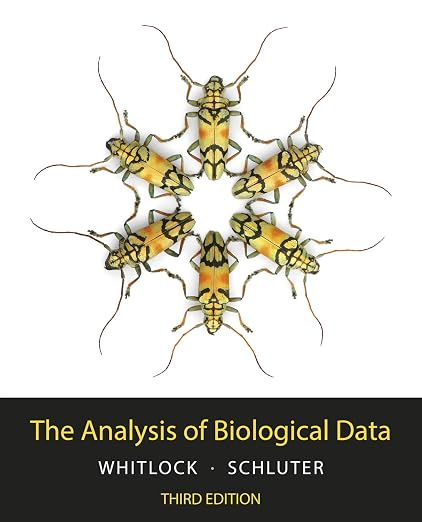
\includegraphics[height=0.3\textheight]{figures/whitlock_book.jpg}
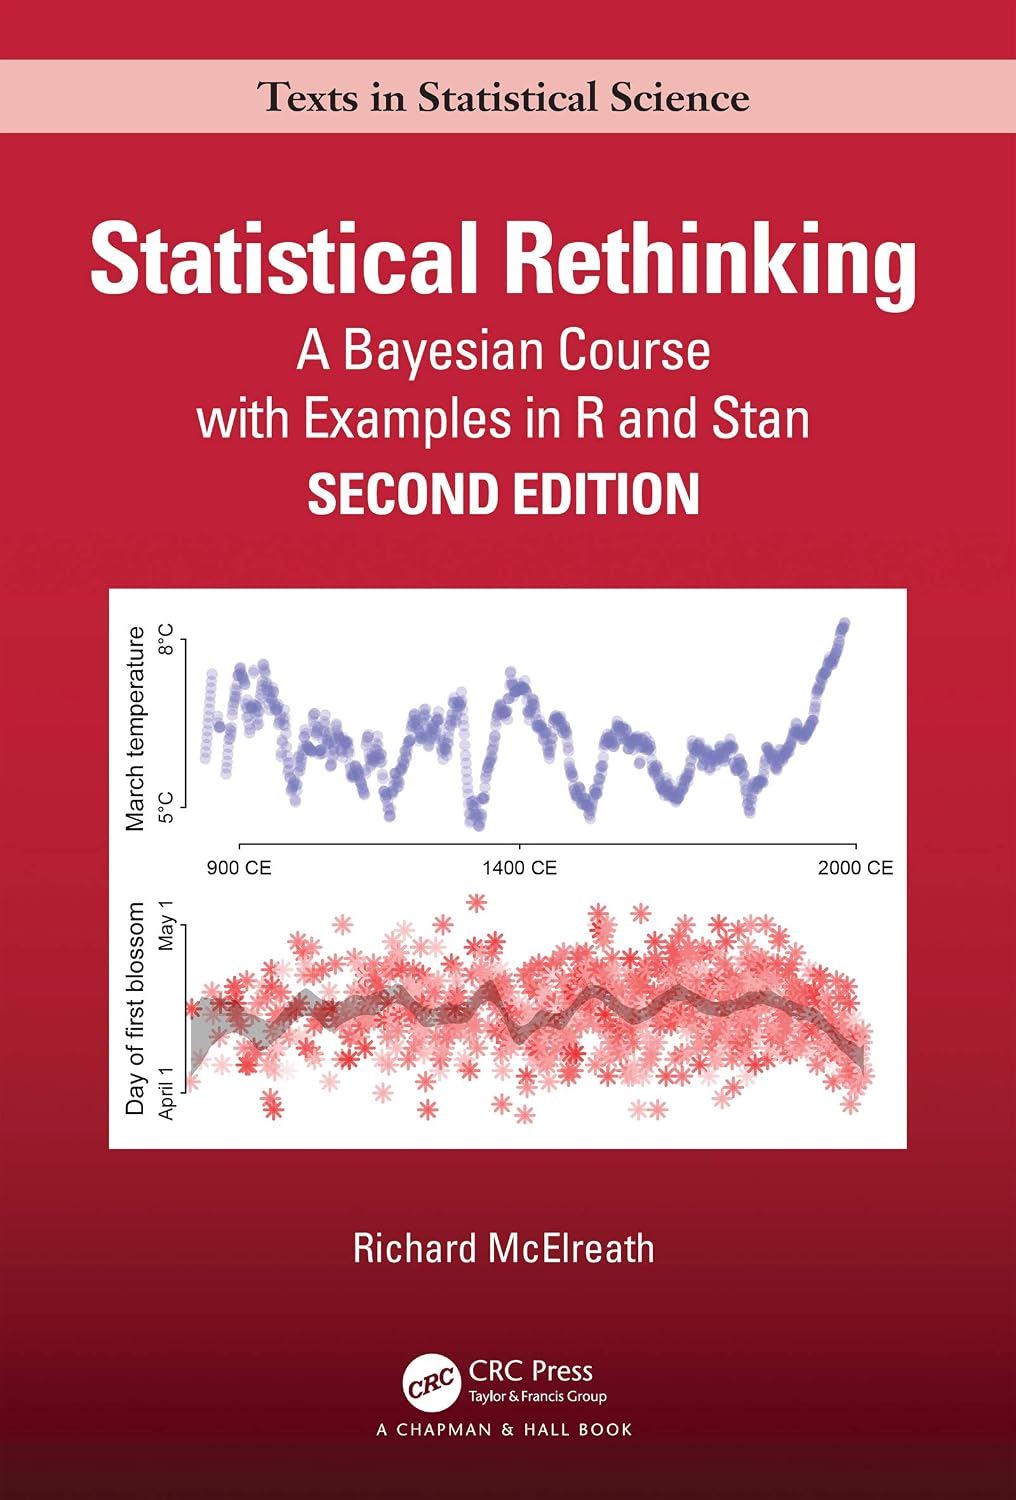
\includegraphics[height=0.3\textheight]{figures/mcelreath_book.jpg}
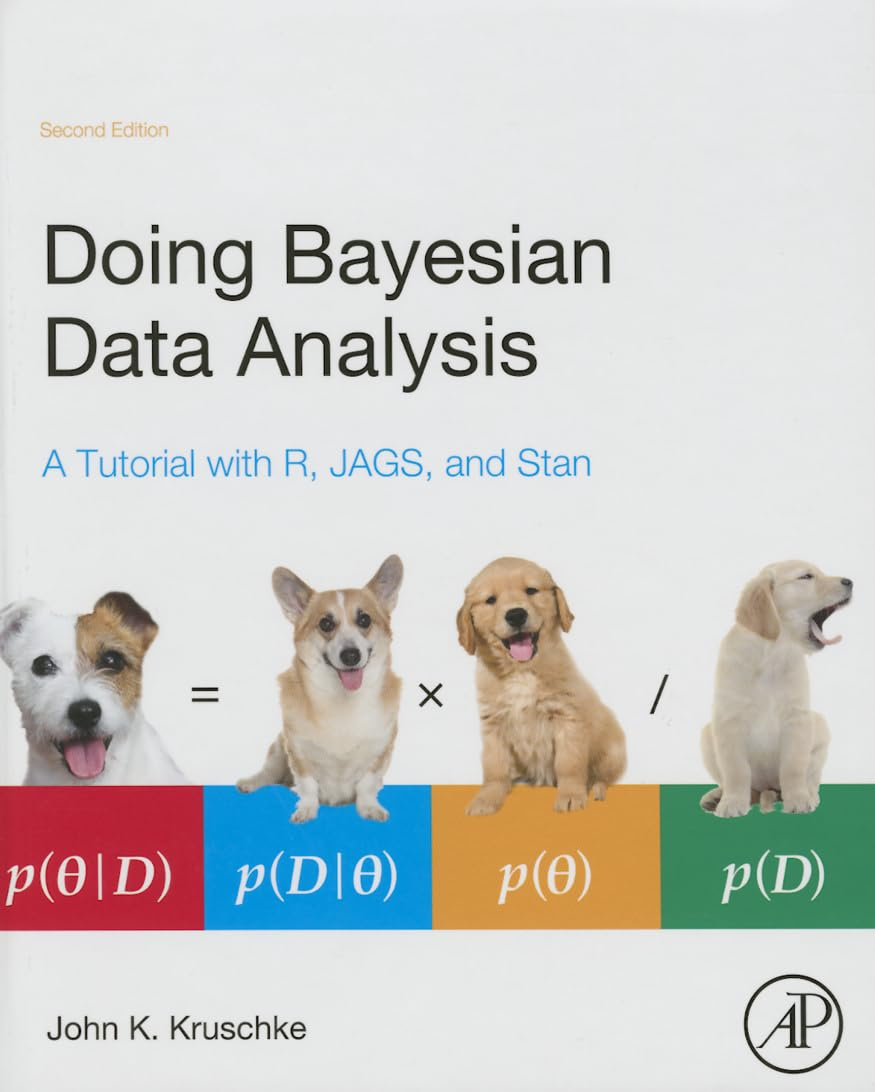
\includegraphics[height=0.3\textheight]{figures/kruschke_book.jpg}
\end{center}

\textbf{NB:}

\begin{itemize}
\tightlist
\item
  all this material is unfortunately behind expensive pay-walls
\item
  even in the age of LLMs, getting solid basics in statistics will make
  you more efficient, critical \& confident
\end{itemize}
\end{frame}

\begin{frame}{Learning more --- statistics and the quest for knowledge}
\protect\phantomsection\label{learning-more-statistics-and-the-quest-for-knowledge}
\begin{itemize}
\tightlist
\item
  watch the excellent video from Veritasium which summarises much of the
  frequentist content from this course\\
  \url{www.youtube.com/watch?v=42QuXLucH3Q}
\end{itemize}

\pause

\begin{itemize}
\tightlist
\item
  accept the fact that much of the research findings is false, but
  contribute to build better science with your newly acquired or
  refreshed statistical knowledge
\end{itemize}

\begin{center}
\begin{figure}
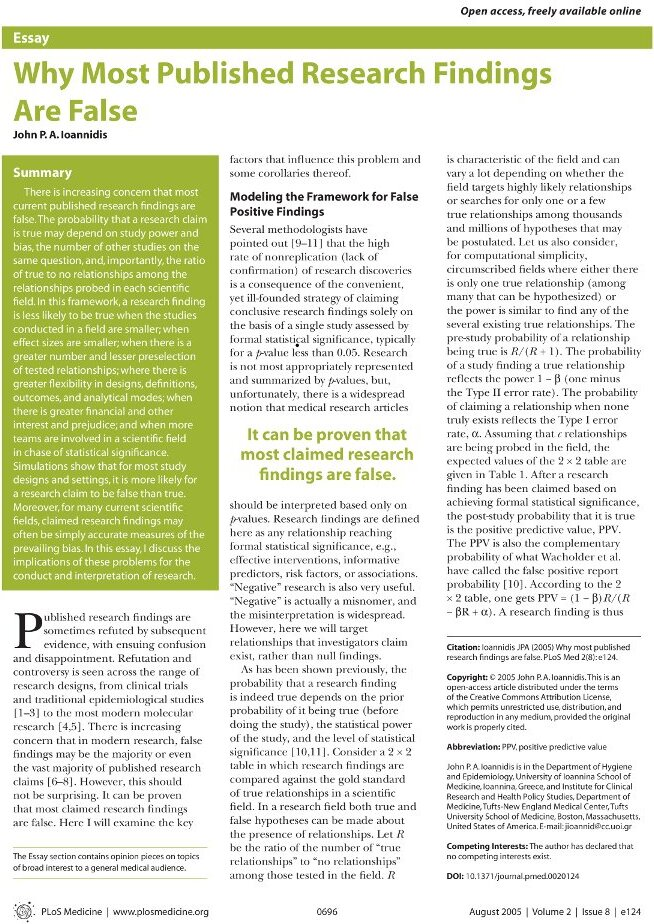
\includegraphics[height=0.4\textheight]{figures/WMPRFAF.jpg}
\caption{\footnotesize Ioannidis (2005) \emph{PLoS Med} 2(8): e124}
\end{figure}
\end{center}
\end{frame}

\section*{Questions?}\label{questions}

\section*{Developer corner}\label{developer-corner}

\begin{frame}[fragile]{Ignore this slide --- (technical info for Alex)}
\protect\phantomsection\label{ignore-this-slide-technical-info-for-alex}
\tiny

\begin{verbatim}
[1] "2.8 min of R running time"
\end{verbatim}

\begin{verbatim}
R version 4.6.1 (2026-06-24)
Platform: x86_64-redhat-linux-gnu
Running under: Fedora Linux 44 (KDE Plasma Desktop Edition)

Matrix products: default
BLAS/LAPACK: FlexiBLAS OPENBLAS-OPENMP;  LAPACK version 3.12.1

attached base packages:
[1] stats     graphics  grDevices datasets  utils     methods   base     

other attached packages:
 [1] nimble_1.4.2       bayesplot_1.15.0   posterior_1.7.0    geomtextpath_0.2.0 lubridate_1.9.5    forcats_1.0.1      stringr_1.6.0     
 [8] dplyr_1.2.1        purrr_1.2.2        readr_2.2.0        tidyr_1.3.2        tibble_3.3.1       ggplot2_4.0.3      tidyverse_2.0.0   

loaded via a namespace (and not attached):
 [1] tensorA_0.36.2.1     gtable_0.3.6         xfun_0.60            lattice_0.22-9       tzdb_0.5.0           numDeriv_2016.8-1.1 
 [7] CoprManager_0.5.8    vctrs_0.7.3          tools_4.6.1          Rdpack_2.6.6         generics_0.1.4       parallel_4.6.1      
[13] proxy_0.4-29         pkgconfig_2.0.3      Matrix_1.7-6         checkmate_2.3.4      RColorBrewer_1.1-3   S7_0.2.2            
[19] distributional_0.8.1 lifecycle_1.0.5      compiler_4.6.1       farver_2.1.2         textshaping_1.0.5    tinytex_0.60        
[25] codetools_0.2-20     htmltools_0.5.9      yaml_2.3.12          pracma_2.4.6         nloptr_2.2.1         pillar_1.11.1       
[31] MASS_7.3-66          reformulas_0.4.4     abind_1.4-8          boot_1.3-32          spaMM_4.6.65         nlme_3.1-170        
[37] tidyselect_1.2.1     digest_0.6.39        stringi_1.8.9        slam_0.1-56          reshape2_1.4.5       labeling_0.4.3      
[43] fastmap_1.2.0        grid_4.6.1           cli_3.6.6            magrittr_2.0.5       utf8_1.2.6           withr_3.0.3         
[49] scales_1.4.0         backports_1.5.1      registry_0.5-1       timechange_0.4.0     rmarkdown_2.31       matrixStats_1.5.0   
[55] igraph_2.3.3         otel_0.2.0           hms_1.1.4            coda_0.19-4.1        ROI_1.0-2            pbapply_1.7-4       
[61] evaluate_1.0.5       knitr_1.51           rbibutils_2.4.1      viridisLite_0.4.3    rlang_1.3.0          isoband_0.3.0       
[67] Rcpp_1.1.2           glue_1.8.1           rstudioapi_0.19.0    minqa_1.2.8          jsonlite_2.0.0       plyr_1.8.9          
[73] R6_2.6.1             systemfonts_1.3.2   
\end{verbatim}

\normalsize
\end{frame}




\end{document}
